\documentclass{book}
%\documentstyle[../LaTex-doc/tr2latex/troffman,makeidx,times,psfig,epsfig,amstex]{book}
\usepackage{times,psfig,epsfig,amstex,./troffman}
\newcommand{\ver}{2.3}
\newcommand{\version}{Version 1.0}
\newcommand{\sciversion}{Version 2.3}

\newcommand{\logical}{{Synchro }}

\newcommand{\computational}{{\em Computational }}
\newcommand{\interfacing}{{\em Interfacing }}

%\markright{ SCICOS - a dynamic system builder and simulator }


%\def\Shead#1{\paragraph{#1}}
%\def\scitem{\begin{itemize}}
%\def\endscitem{\end{itemize}}
%\def\endscitem{\end{itemize}}

\makeatletter

\title{SCICOS\\[.1cm]
{A Dynamic System Builder and Simulator}\\[.4cm]
User's Guide - \version}
\author{R. Nikoukhah \and S. Steer}
\date{\input demo2.tex
}



\begin{document}

\maketitle

\chapter*{Preface}
The development of Scicos is part of the ongoing project ``Scilab'' at
INRIA 

\begin{center}
Institut National de Recherche en Informatique et en Automatique \\
Rocquencourt, BP 105 \\
78153 Le Chesnay Cedex, France
\end{center}

All the programs developed in this project are distributed free, with all
the sources, through Internet and other media.

\bigskip

Scicos (Scilab Connected Object Simulator) is a Scilab package for
modeling and simulation of hybrid dynamical systems. 
More specifically, Scicos is intended to be a simulation environment in which 
both continuous systems and discrete systems co-exist. Unlike many
other existing hybrid system simulation softwares, Scicos has not
been constructed by extension of a continuous simulator or of a
discrete simulator; Scicos has been developed based on a formalism
that considers both aspects from the beginning. 
Scicos includes a graphical editor which can be used to build complex
models by interconnecting blocks which represent either predefined basic
functions defined in Scicos libraries (palettes), or user defined
functions. A large class of hybrid systems can be modeled and
simulated this way.

\bigskip 

The objective of the development of Scicos is along the lines of that
of Scilab, that is to provide the scientific community with a
a completely open and free environment for scientific computing. 
Just like Scilab, Scicos is more than just a research tool, it has
already been used in a number of
industrial projects. Even though its applications so far have been
mostly limited to the areas of control and signal processing, Scicos, and
specially this new version of it, should find other applications in other areas.

\bigskip 


This version of Scicos is a built-in library (toolbox) of Scilab \ver. 
For information on Scicos and Scilab in
general, consult {\tt http://www-rocq.inria.fr/scilab} and newsgroup 
{\tt comp.soft-sys.math.scilab}. The latest version of Scilab can be
obtained by anonymous ftp from {\tt ftp.inria.fr}. The source code
and binary versions for various platforms can be found in the directory
{\tt /INRIA/Scilab}.


\tableofcontents
\listoffigures
\listoftables

\chapter{Introduction}
Even though it is possible to simulate mixed discrete and
continuous (hybrid) dynamics systems in Scilab using Scilab's ordinary
differential equation solver (the {\tt ode}
function), implementing the discrete  recursions and the logic for
interfacing the discrete and the continuous parts usually
requires a great deal of programming. These programs are often
complex, difficult to debug and slow. 


There have been a number of models proposed in the literature for
hybrid dynamical systems (see for example \cite{Hybrid,mats}). 
A simple, yet powerful model is the following:
\begin{eqnarray}
\dot{x} &=& f(x) \label{ett1} \\
\mbox{if}\;\;h_i(x)=0,&&\mbox{then}\;\;x:=g(i,x) ,\;i=1,2,...,m, \label{ett2}
\end{eqnarray}
where $x\in \mathbb{R}^n$ is the state of the system, $f$ is a vector
field on $\mathbb{R}^n$, $g$ is a mapping from $\mathbb{N}\times \mathbb{R}^n
\rightarrow \mathbb{R}^n$ and $h_i$'s are continuous
functions. (\ref{ett2}) should be interpreted as: when $h_i(x)$ crosses
zero, the state jumps from $x$ to $g(i,x)$; and of course, between two
state jumps, (\ref{ett1}) describes the evolution of the system. The
zero crossing of $h_i(x)$ is referred to as an event $i$. An event
then causes a jump in the state of the system.

This model may seem very simple, yet it can model many interesting
phenomena. Consider for example the dependence on time. It may seem that
(\ref{ett1})-(\ref{ett2}) cannot model time-dependent systems. This,
however, can be done by state augmentation. For that it suffices to
add $\dot{t}=1$ to system equations and augment the state by adding $t$ to it. 

To model discrete-time systems, i.e., systems that evolve according to
\begin{equation}
\xi(k+1)=f(k,\xi(k)),
\end{equation}
first, an event generator is needed. A simple event generator would be
\begin{eqnarray}
\dot{e}&=&-1  \\ \label{ett3}
\mbox{if}\;\;e=0,&&\mbox{then}\;\;e:=1.
\end{eqnarray}
So $e$ starts off as $1$ and with constant slope
of $-1$, it reaches zero one unit of time later. At this point, an
event is generated and $e$ goes back to $1$ and the process starts
over. These events can then be used to update $\xi$. The complete
system would then be:
\begin{eqnarray}
\dot{k}&=&0 \\
\dot{\xi}&=&0 \\
\dot{e}&=&-1 \\
\mbox{if}\;e=0,&&\mbox{then}\;\;e:=1,\xi:=f(k,\xi),k:=k+1.
\end{eqnarray}

State augmentation is a nice way of modeling hybrid systems in the form 
(\ref{ett1})-(\ref{ett2}), however, it is in most cases not useful for
the purpose of simulation. It is clearly too costly to integrate
(\ref{ett3}) for realizing an event generator, or integrate $1$ to
obtain $t$. Even for model construction, (\ref{ett1})-(\ref{ett2})
does not provide a very useful formalism. To describe hybrid models in
a reasonably simple way, a richer set of operators need to be used
(even if they can all, at least in theory, be realized by state
augmentation as (\ref{ett1})-(\ref{ett2})).
Scicos proposes a fairly rich set of
operators for modeling hybrid systems from a modular description. The
modular aspect (possibility of constructing a model by
interconnection of other models) introduces additional complexity
concerning, mainly, event scheduling and causality. 

\bigskip

Scicos basic operators suffice to model many interesting problems
in systems, control and signal processing applications. 
Scicos editor provides an easy to use graphical editor for building complex
models of hybrid systems in a modular way, a compiler which converts
the graphical description into Scicos executable code, and a simulator.
The simple session presented in Chapter~\ref{ch2},
the examples of Chapter~\ref{ch6} 
and specially the demos provided with the package, should allow new
users to start building and simulating simple models very quickly. It
is however recommended that users familiarize
themselves with basic concepts and elementary building blocks of
Scicos by reading Chapters~\ref{ch4}, \ref{ch5} and, at least the
first section of Chapter~\ref{Evaluation}. 

\bigskip

Scicos  \version\ is still a beta test version; 
it has not been fully tested.
Questions, discussions and suggestions should be posted to newsgroup 
\begin{center}
{\tt comp.soft-sys.math.scilab}
\end{center}
and bug reports should be sent to {\tt scilab@inria.fr}.



\chapter{Getting started}
\label{scasm}
\label{ch2}
This section presents the steps required for modeling and simulating a simple
dynamic system in Scicos. In Scicos, systems are modeled in a modular way
by interconnecting subsystems referred to as {\em blocks}. The model we
construct here uses
only existing blocks (available in various palettes); the procedure for creating
new blocks will be discussed later.

\section{Constructing a simple model}
In Scilab main window, type \underline{{\tt scicos();}}. This opens up an empty Scilab graphic
window with a menu bar on the side (Figure \ref{fig0}). By default, this window is
named {\tt Untitled}. 
  \begin{figure}[hbtp]
  \centerline{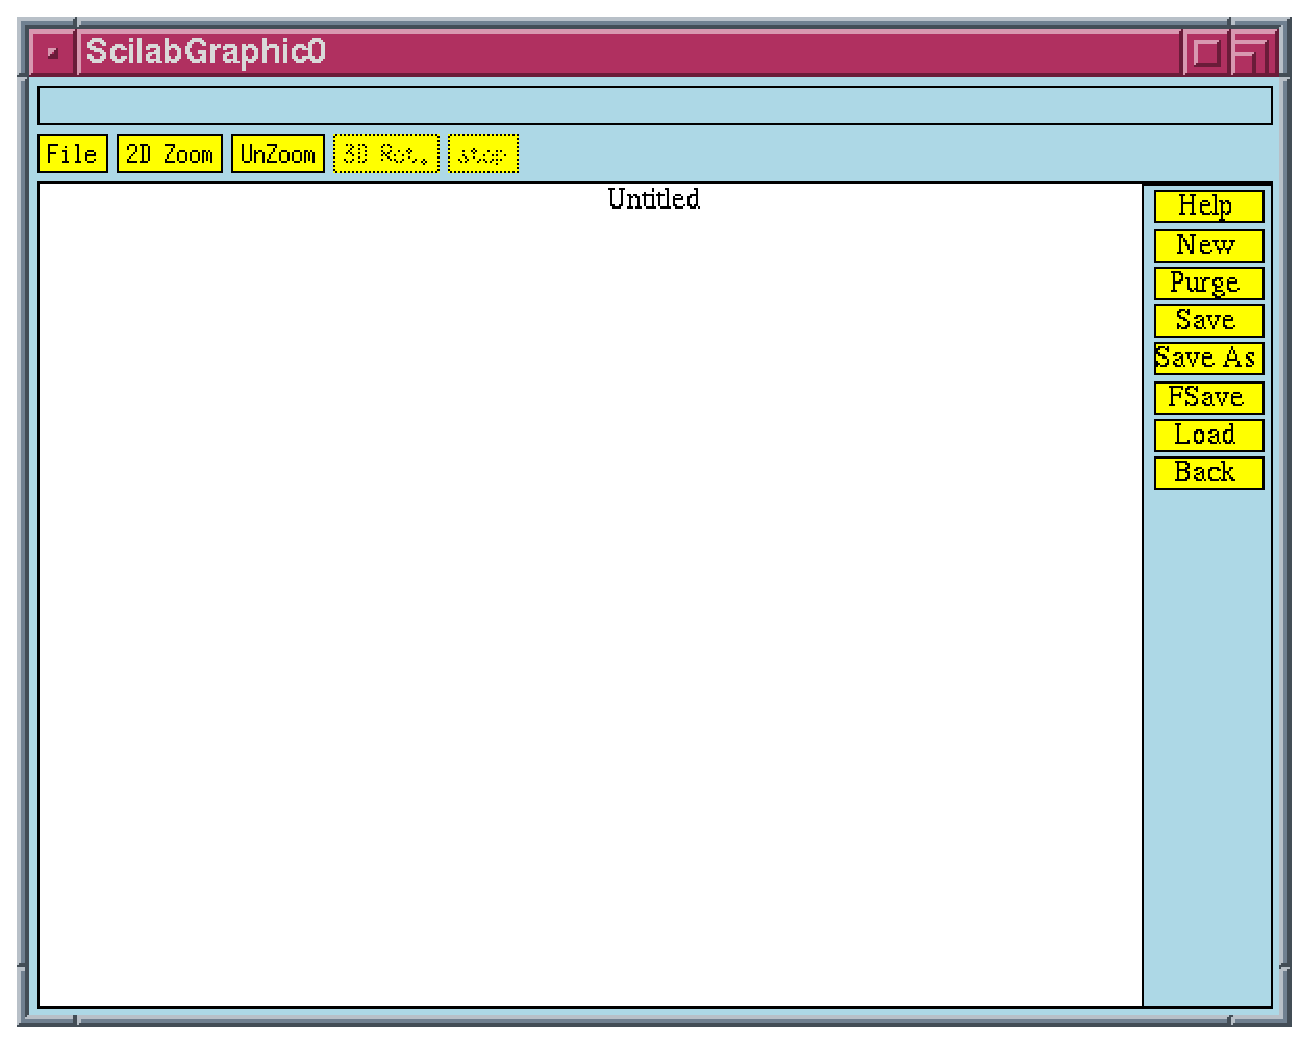
\epsfig{file=xwfig0.eps,width=11cm}}
  \caption{Scicos main window}
 \label{fig0}
  \end{figure}

Click on the {\tt Edit..} button to obtain the {\tt Edit} menu bar.
To open up a palette, click on the {\tt Palettes} button. 
You are then presented with a choice of palettes (Figure \ref{choice1}).
Click on {\tt Inputs/Outputs}; this opens up a palette which is a
new Scilab graphic window containing
a number of blocks (Figure~\ref{pal1}). To copy a block, click first on the {\tt copy}
button in Scicos main window, then on the block to be copied in the
palette, and finally somewhere
in the Scicos main window, where the block is to be placed. 
  \begin{figure}[hbtp]
  \centerline{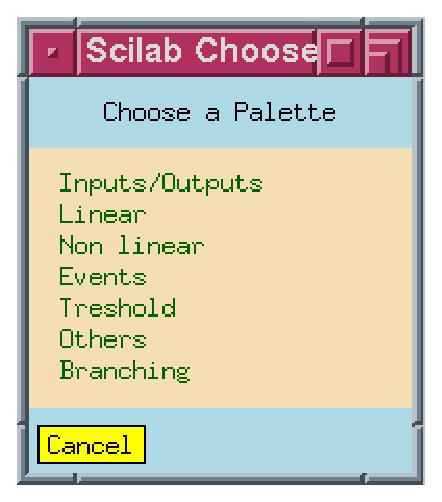
\epsfig{file=xwchoice1.eps,width=5cm}}
  \caption{Choice of palettes}
 \label{choice1}
  \end{figure}

\input pal1.tex
\dessin{Inputs/Outputs Palette}{pal1}

Using this procedure, copy the {\tt MScope} block, 
the {\tt sinusoid generator} block and the
{\tt Clock} block (the clock with an output port on the bottom) 
into Scicos main window.
The result should look like in Figure~\ref{gogo2}.
\input gogo2.tex
\dessin{These blocks have been copied from the Inputs/Outputs Palette}{gogo2}

Open the {\tt Linear} palette and copy the block {\tt 1/s} (integrator) into
Scicos main window. Connect the input and output ports of the blocks
by clicking first on the {\tt link} button, then on the output port and then on the
input port (or on intermediary points if you don't just want 
a straight line connection), for each new link.
Connect the blocks as illustrated in Figure~\ref{gogo3}. To make a path originate 
from another path, i.e., be split, click
on the {\tt Link} button and then on an existing path, where split is
to be placed, and finally on an input port (or intermediary points
before that). 


\input gogo3.tex
\dessin{Complete model}{gogo3}

\bigskip 

The {\tt Clock} generates a train of impulses which tells the {\tt MScope}
block at what times the value of its inputs must be displayed. To inspect (and if needed change)
the {\tt Clock} parameters, click on the {\tt Clock} block. 
This opens up a dialogue panel
as illustrated in Figure~\ref{gogo4}. At this point the period, i.e. the time period
between events and the time of the first event can be changed. 
Let's leave them unchanged;
click on {\tt Cancel} or {\tt OK}. Similarly you can inspect the parameters of other
blocks. You can now save your diagram by clicking on the {\tt Save} button. This saves
your diagram in a file called {\tt Untitled.cos} in the directory where Scilab was
launched. 
  \begin{figure}[hbtp]
  \centerline{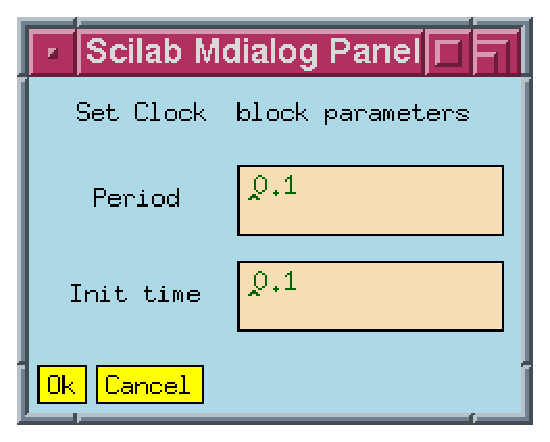
\epsfig{file=xwgogo4.eps, width=6cm}}
  \caption{{\tt Clock}'s dialogue panel}
 \label{gogo4}
  \end{figure}

\section{Model simulation} 
It is now time to do a simulation. For that you need to 
leave the {\tt Edit..} menu; click
on {\tt back}. You are now back to the main menu. Click on {\tt Simulate..}, you have now
the simulation menu. Click on {\tt Run}. After a short
pause (time of compilation), the simulation starts; see Figure~\ref{gogo9}.


The simulation can be stopped by clicking on the {\tt stop} button on top of the Scicos main
window. It is clear at this point that the {\tt MScope}'s parameters need to be adjusted.
So, click on the {\tt MScope} block; this opens up a dialogue box (see Figure~\ref{gogo71}).
\input gogo9.tex
\dessin{Simulation result}{gogo9}

Clearly to improve the display, we must change {\tt Ymin} and {\tt
Ymax} of the two 
plots.
The first input ranges from 0 to 2 and the second form -1 to 1; {\tt
Ymin} and {\tt Ymax}
can now be adjusted accordingly. Increasing the {\tt Buffer size} 
can speed up the simulation,
but can make the display "jerky". The refresh period is the maximum 
time displayed in a single window. We can also change the colors of 
the two curves. Modify the parameters in 
the dialogue box as in Figure~\ref{gogo8}.
  \begin{figure}[hbtp]
  \centerline{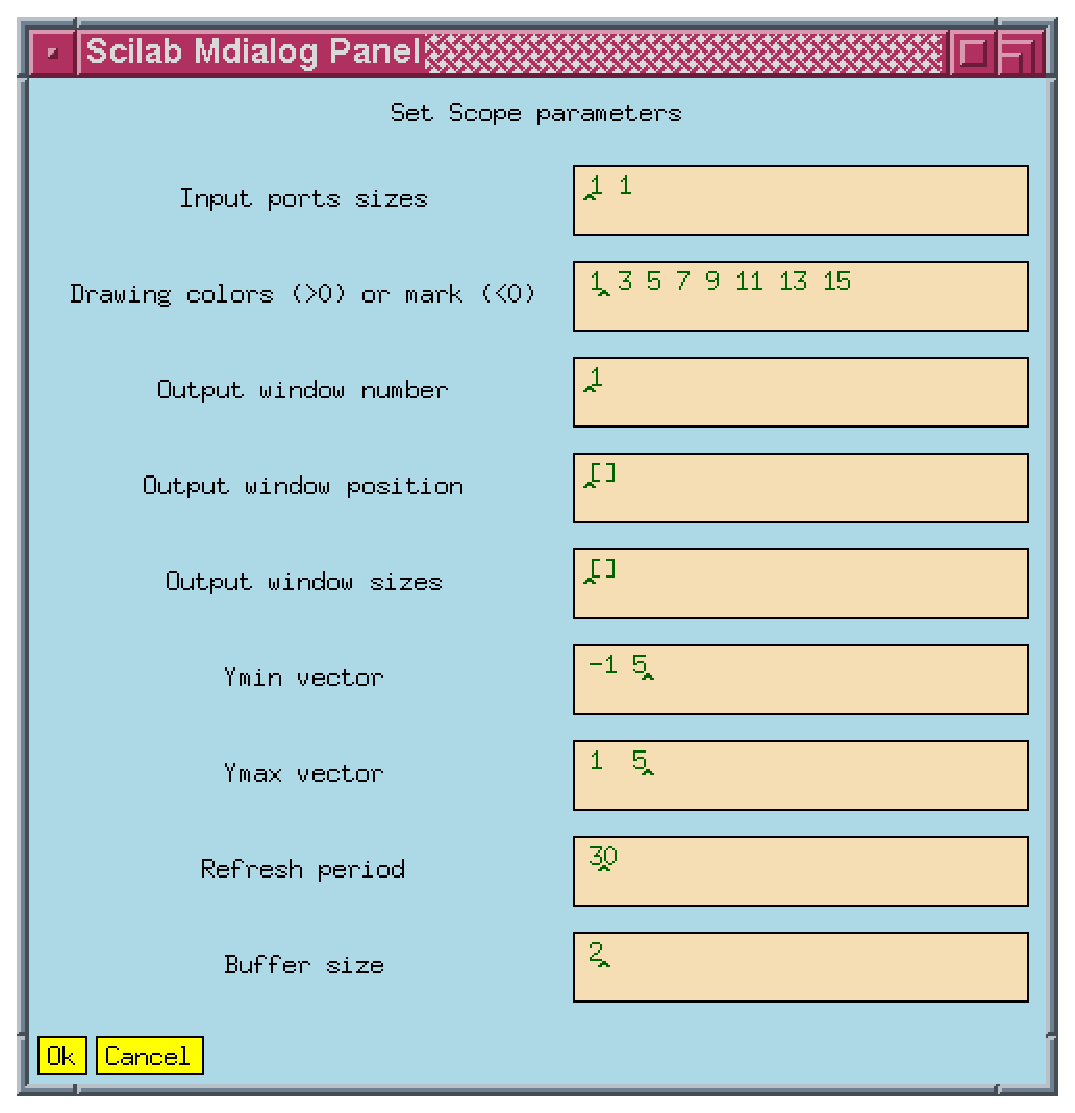
\epsfig{file=xwgogo7.eps,width=11cm}}
  \caption{{\tt MScope} original dialogue box}
  \label{gogo71}
  \end{figure}

Click now on {\tt OK} to register the new parameters and get back to the Scicos main window.
You can now restart the simulation by clicking on {\tt Run} and 
selecting {\tt Restart} among the proposed choices. The result is
depicted in Figure~\ref{gogo9}. Note that
this time the simulation starts right off, no need for re-compilation.
  \begin{figure}[hbtp]
  \centerline{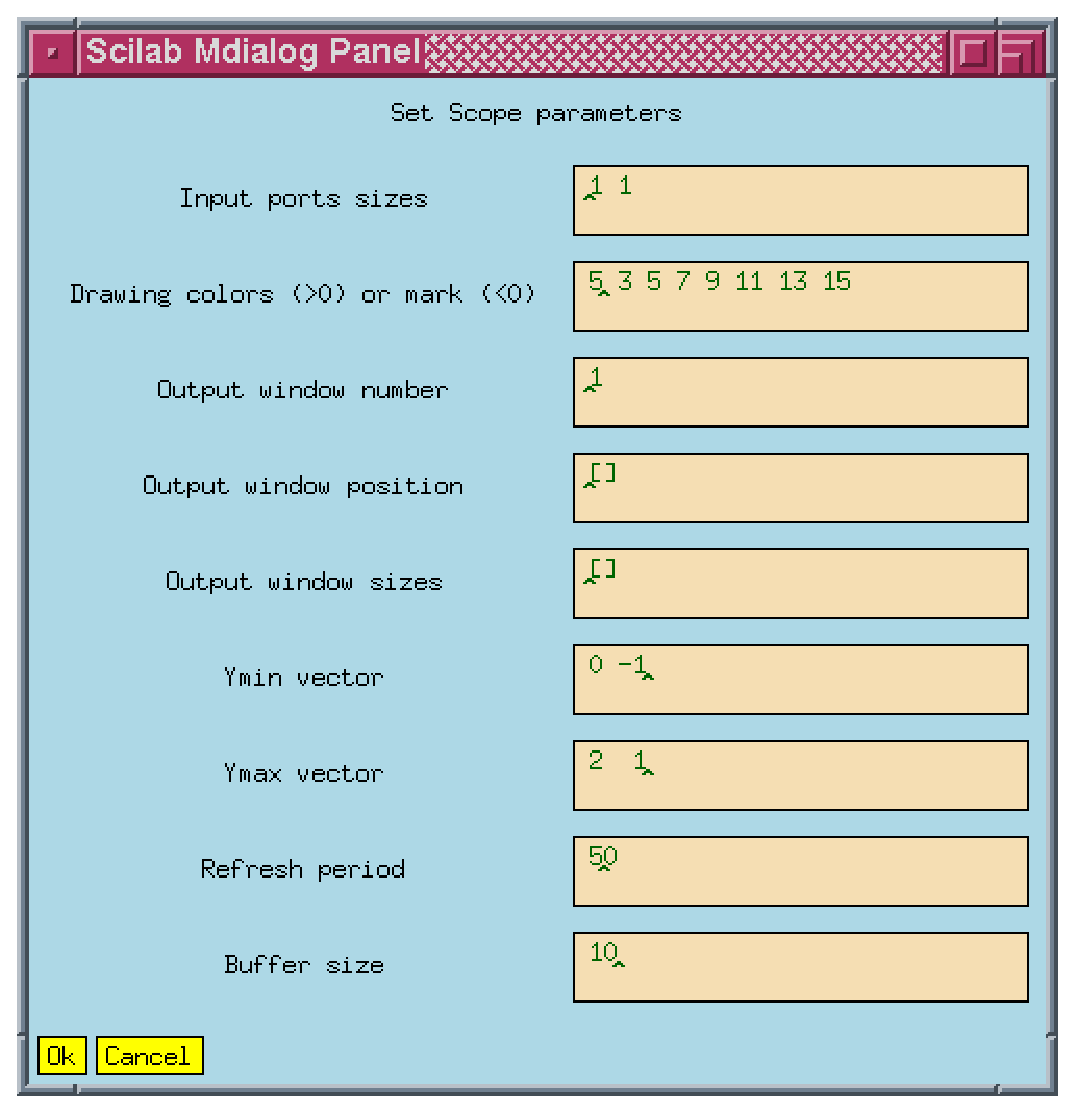
\epsfig{file=xwgogo8.eps,width=11cm}}
  \caption{{\tt MScope} modified dialogue box}
 \label{gogo8}
  \end{figure}

\input gogo7.tex
\dessin{Simulation result after modifications}{gogo7}

\bigskip

To make your diagram look good, you can go back to the main menu and 
click on {\tt Block..}. Here you can change the background colors of the blocks
({\tt Color}), the texts or pictures displayed inside them ({\tt Icon}) and their
sizes ({\tt Resize}). For example to color the block MScope, click on the
button {\tt Color}, then on the block. This opens up a color palette; 
select the desired color by clicking on it, and confirming by {\tt OK}.
To change the color of a link, simply click on it.

You can also place text on your diagram by copying the block {\tt Text} in
{\tt Others} palette into your diagram and changing the text, the font and
the size by clicking on it.

Finally, you can print and export, in various formats, your diagram using
the {\tt File} menu on top of the corresponding graphics window. Make
sure to do a replot before to clean up the diagram. The result will be
like the diagrams in this document. 

\section{Symbolic parameters and ``context''}
\label{symb}
In the above example, the block parameters seem to be defined numerically. 
But in fact, even when a number is entered
in a block's dialogue, it is first treated and memorized symbolically, and
then evaluated. For example in the block {\tt sinusoid generator}, we can
enter {\tt 2-1} instead of {\tt 1} for {\tt Magnitude} and the result would be the same
(see Figure ~\ref{para1}); opening
up the dialogue the next time around would display {\tt 2-1}. We can go
further and for example use a symbolic expression such as {\tt sin(cos(3)-.1)}.


  \begin{figure}[htbp]
  \centerline{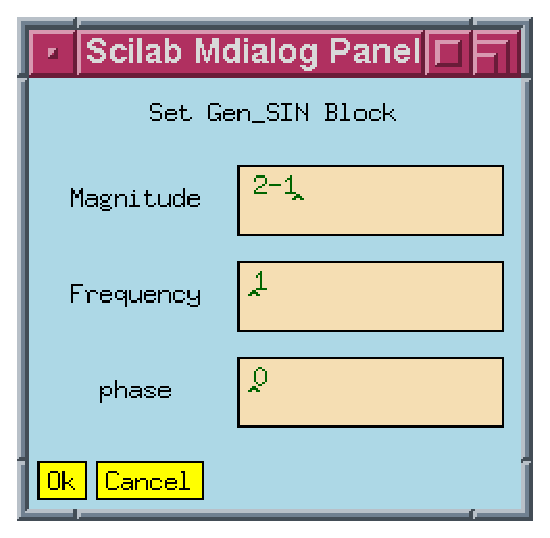
\epsfig{file=xwpara1.eps,width=6cm}}
  \caption{Symbolic expression as parameter}
 \label{para1}
  \end{figure}

In fact we can use any valid Scilab expression, including Scilab variables. But,
these variables (symbolic parameters) should be defined at some point. For that
click on the {\tt context} button in the 
{\tt edit} menu. You are then
presented with a ``Dialogue Panel'' (see Figure~\ref{ampl}) in which you
can define symbolic parameters (in this case {\tt ampl}). Once you
click on {\tt OK}, the variable {\tt ampl} can be used in all the
blocks in the diagram. It can for example be used to change, in {\tt sinusoid generator} block,
the magnitude of the sine-wave (see Figure~\ref{ampl2}).


  \begin{figure}[htbp]
  \centerline{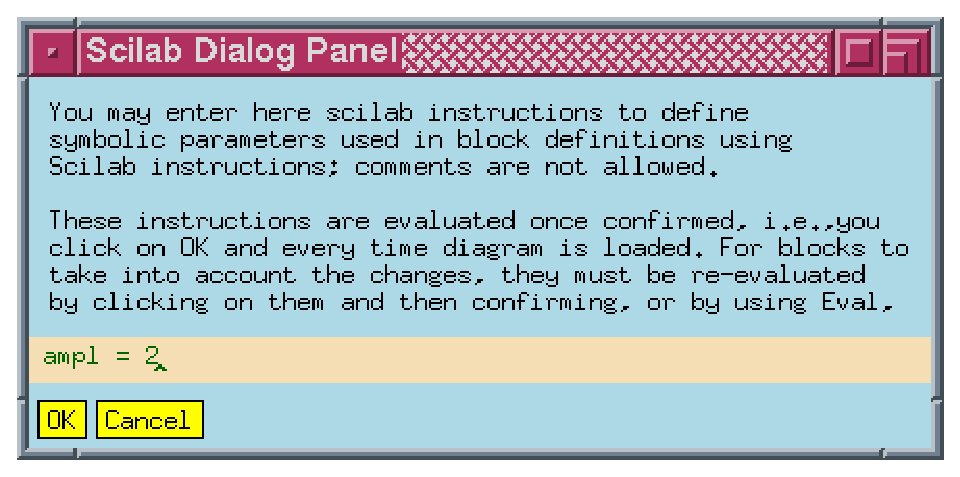
\epsfig{file=xwampl.eps,width=11cm}}
  \caption{Context is used to give numerical values to symbolic expressions}
 \label{ampl}
  \end{figure}

  \begin{figure}[htbp]
  \centerline{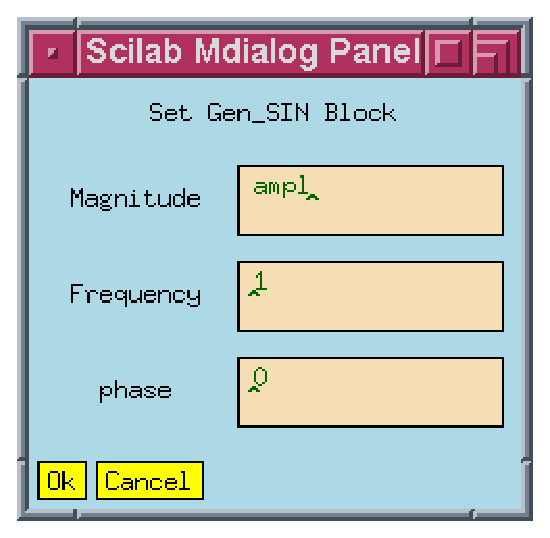
\epsfig{file=xwampl2.eps,width=6cm}}
  \caption{Use of symbolic expressions in block parameter definition}
 \label{ampl2}
  \end{figure}

The context of the diagram is saved with the diagram and the expressions
are re-evaluated when the diagram is reloaded. Note however that if you
change the context, you must re-evaluate the diagram if you want the
blocks to take into account the changes. That can be done either by
clicking on the {\tt eval} button in the {\tt Simulate} menu, or by
clicking on the concerned blocks and confirming.

\section{Use of Super Block}
It would be very difficult to model a comlex system with hundreds of
component in one diagram. For that, Scicos provides the possibility
of grouping blocks together and defining sub-diagrams called Super Blocks.
These blocks have the appearance of regular blocks but can contain
an unlimited number of blocks, even other Super Blocks. A Super Block can be
duplicated using the {\tt copy} button in the {\tt Edit} menu and used any
number of times.

\input supi.tex
\dessin{Super Block in the diagram}{supi}


To define a Super Block, copy {\tt Super Block} from {\tt Others} palette
into your diagram (see Figure~\ref{supi}) and click on it. This opens up
a new Scicos panel with an empty diagram. Edit this diagram by copying and connecting a 
{\tt S/H} block (sample and hold), a discrete linear system, and
input and output Super Block ports as in Figure~\ref{supi2}.


\input supi2.tex
\dessin{Super Block content}{supi2}

Once you exit (using {\tt Exit} button) from the Super Block panel, you
get back to the original diagram. Note that the Super Block now has the
right number of inputs and outputs, i.e., one event input port on top,
one regular input port and one regular output port. To drive this discrete
component, we need a {\tt Clock}; just copy the {\tt Clock} already in
the diagram (see Figure~\ref{supi3}). Note that there is no need to
disconnect the links to {\tt MScope} to change the number of its inputs.
Simply update its parameters as in Figure~\ref{supi4}; the input ports adjust
automatically. 


\input supi3.tex
\dessin{Complete diagram with Super Block}{supi3}


  \begin{figure}[htbp]
  \centerline{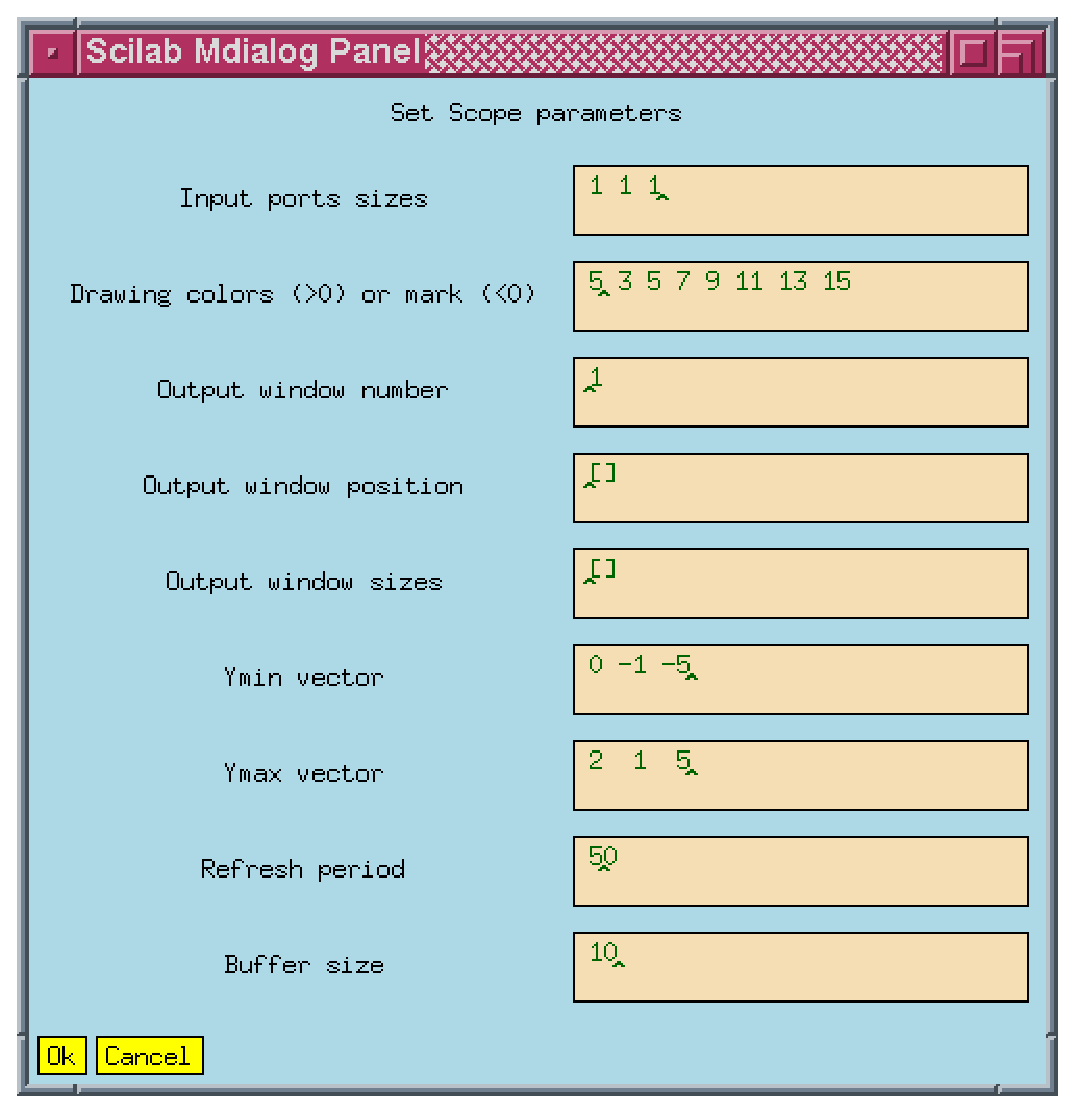
\epsfig{file=xwsupi4.eps,width=11cm}}
  \caption{MScope updated dialogue box}
 \label{supi4}
  \end{figure}

Before simulating, set the period of this new {\tt Clock} to 2 (to observe
the discrete behavior, period of discretization must be larger than that of
the scope). You can now {\tt Run} the diagram.


\chapter{Basic concepts}
\label{ssa}
\label{ch4}
Models in Scicos are constructed by interconnection of Basic
Blocks. There exist four types of Basic Blocks and two types of
connecting paths (links) in Scicos. Basic Blocks can have two types of
inputs and two types of output: regular inputs, event inputs, regular
outputs and event outputs. Regular inputs and outputs are
interconnected by regular paths, and event inputs and outputs, by
event paths (regular input and output ports are placed on the sides of
the blocks, event input ports are on top and event output ports are on
the bottom). Blocks can have an unlimited number of each type of input
and output ports).

Regular paths carry piece-wise right-continuous functions of time
whereas event paths transmit timing information concerning discrete
events.\footnote{Regular paths are vectorized in a sense that each
link can carry  
a set of functions; event links are not.}
One way to think of event signals as physical signals is to
consider them as impulses, so in a sense event paths transmit
impulses from output event ports to input even ports. To see how event
signals (impulses) are generated and how they affect the blocks, a
look at the behaviors of Basic Blocks is necessary.



\section{Basic Blocks}
There are four types of Basic Blocks in Scicos.

\subsection{Continuous Basic Block}
Continuous Basic Blocks (CBB) can have both regular and event input and output
ports. CBB's can model more than just continuous 
dynamics systems. A CBB can have a {\em continuous state} $x$ and a 
{\em discrete state}
$z$. Let the vector function $u$ denote the regular inputs and $y$ the regular
outputs. Then a CBB imposes the following relations
\begin{eqnarray}
\dot{x} &=& f(t,x,z,u,p) \label{e1}\\
y&=&h(t,x,z,u,p) \label{e2}
\end{eqnarray}
where $f$ and $h$ are block specific functions, and $p$ is a vector of
constant parameters. Constraints (\ref{e1})-(\ref{e2}) are imposed by
the CBB as long as no events (impulses) arrive on its event input ports. An
event input can cause a jump in the states of the CBB. Let's
say one or more events  arrive on  CBB's event ports at time $t_e$, then
the states jump according to the following equations:
\begin{eqnarray}
x &:=& g_c(t_e,x(t_e^-),z(t_e^-),u(t_e^-),p,n_{evprt}) \label{e11}\\
z &:=& g_d(t_e,x(t_e^-),z(t_e^-),u(t_e^-),p,n_{evprt}) \label{e12}
\end{eqnarray}
where $g_c$ and $g_d$ are block specific functions; $n_{evprt}$ 
designates the port(s)
through which the event(s) has (have) arrived; ${x}$ and ${z}$ are
the vectors of continuous state and
discrete state. $z(t_e^-)$ is the previous value of the discrete state $z$;
$z$ remains constant between any two successive events. 

\begin{figure}[ht]
\input test1.pstex_t
\caption{A Continuous Basic Block}
\label{cbb}
\end{figure}


Finally, CBB's can generate event signals on their event output
ports. These events can only be scheduled at the arrival of an input
event. If an event has arrived at time $t_e$, the time of each output event 
is generated according to
\begin{equation}
t_{evo} := k(t_e,z(t_e),u(t_e),p,n_{evprt})  \label{e20}
\end{equation}
for a block specific function $k$ and where $t_{evo}$ is a vector of
time, each entry of which corresponds to one event output port. Normally all
the elements of $t_{evo}$ are larger than  $t_e$. If an
element is less than $t_e$, it simply means the absence of an output
event signal on the corresponding event output port. $t_{evo}=t$
should be avoided, the resulting causality structure is ambiguous.
Note that even if
$t_{evo}=t$, this does not mean that the output event is synchronized
with the input event; synchronization of two events is a very restrictive
condition (see \logical
blocks). Two events can have the same time but not be synchronized.

Event generations can also be pre-scheduled. In most cases, if no event
is pre-scheduled, nothing would ever happen (at least as far as events are
concerned). Pre-scheduling of events can  be done by setting the "initial 
firing" variable of each CBB with event output ports. 
Initial firing is a vector with as many 
elements as the block's output event ports. Initial firing can be
considered as the initial condition for $t_{evo}$. By setting  the
$i$-th entry of the initial firing vector to $t_i$, an output event is
scheduled on the $i$-th output event port of the block at time $t_i$ if
$t_i\ge 0$; no output event is scheduled if $t_i<0$. This event is
then fired when time reaches $t_i$.

Only one output event can be scheduled on each output
event port, initially and in the course of the simulation, this means
that by the time a new event is to be scheduled, the old one must have been
fired. This is natural because the register that contains firing
schedule of a block should be considered as part of the state, having
dimension equal to the number of output event ports. 
Another
interpretation is that as long as the previously scheduled event has
not been fired, the corresponding output port is considered busy, meaning it cannot
accept a new event scheduling. If the simulator encounters such a 
conflict, it stops and returns the error message {\em event
conflict}. 

\bigskip

In the unlikely event that a block receives two (or more)
successive events having the same time (without them being
synchronized). For the
second event, the $t_e^-$ should be interpreted as {\em previous value of}.
Note that in that case, the values of $x$ and $u$ at $t_e$ and $t_e^-$ are not uniquely defined;
this means that the time $t$ is not the proper independent variable in terms
of which we should express system's equations but rather a more general concept
of time such as the time of simulation should be used. 
Expressed in such a time frame, 
at the arrival of one or more events at time $t_e$, the variable $t$ freezes 
and the states are updated and then $t$ goes on. 



\subsection{Discrete Basic Block}
The CBB monitors permanently its inputs and updates continuously its
outputs and continuous state. In 
contrast, Discrete Basic Blocks (DBB) act only when they receive an input
event and their actions are instantaneous. 
DBB's can have both regular and event input and output
ports but they must have at least one event input port. DBB's can model discrete 
dynamics systems. A DBB can have a discrete state
$z$ but no continuous state. Let $u$ denote the regular inputs and $y$ the regular
outputs, then, upon the arrival of an event (or events) at time $t_e$, 
the state and the outputs of a DBB change as follows
\begin{eqnarray}
z&:=& f_d(t_e,z(t_e^-),u(t_e^-),p,n_{evprt})  \label{e520} \\
y&:=&h_d(t_e,z,u(t_e),p) \label{e530}
\end{eqnarray}
where $f_d$ and $h_d$ are block specific functions, and $p$ is a vector of
constant parameters and $n_{evprt}$ designates the port(s)
through which the event(s) has (have) arrived.
Needless to say that $y$ remains constant between any two successive
events so that the output $y$ and the state $z$ are
piece-wise constant, right-continuous functions of time.
Like CBB's, DBB's can generate output events according to (\ref{e20}). These
events can also be initialized as in the case of CBB's.


\begin{figure}[ht]
\input test2.pstex_t
\caption{A Discrete Basic Block}
\label{dbb}
\end{figure}


The difference between a CBB and a DBB is that a DBB cannot have a continuous
state and that its outputs remain constant between two events. It is
very simple to emulate a DBB by a CBB, so why a use a DBB? The reason is that
by specifying the block to be a DBB, the simulator knows that the outputs
of this block remain constant between events and uses this information
to optimize simulation performance.

Note that the regular output signal of a DBB is always
piece-wise constant (we refer to it as discrete signal). Being
piece-wise constant does not imply necessarily that a signal is
discrete, for example the output of an integrator (which is a CBB with
continuous state) can in some special cases be constant; the discrete
property characterizes signals that are piece-wise constant based
solely on
the basic properties of the blocks that generate them. In particular,
in Scicos, every regular 
output signal of a DBB is discrete and every regular output signal of
a state-less time invariant CBB receiving only discrete signals on
its inputs is also discrete. Thus, the  discrete nature of signals in a model can be
specified off-line; the compiler does this and uses this information
to optimize simulation performance.

\bigskip

Most of the elementary blocks in Scicos are either CBB's or DBB's: the
followings are a few examples.

\paragraph{Static blocks}
A static block is one where the (regular) outputs are static functions
of its inputs. For example the block that "realizes" $y=\sin(u)$ is a
static block. Static blocks have no input or output event ports, and
they have no state. Clearly these blocks are special cases of CBB's. 

Even though Static blocks are CBB's, they can be used even in
purely discrete models. It is of course possible to construct static
DBB's (i.e.  blocks that realize static functions of their inputs on
their outputs only when events are received on their event input
ports) but it turns out that a 
static DBB does not necessarily perform any better than a static CBB
if its inputs are discrete signals. In particular, knowing the
discrete nature of its inputs, the compiler does not make useless
repeated calls to the static CBB, it makes only one call every time one
of the inputs jumps.

\bigskip

The {\tt Non linear} palette contains a number of
examples of Static blocks.

\paragraph{Discrete-time state-space systems}
A discrete-time system
\begin{eqnarray}
\xi(k+1)&=&m(\xi(k),u(k)) \\
y(k)&=&n(\xi(k),u(k))
\end{eqnarray}
can be implemented as a DBB if the block
receives, on its event input port, event signals on a regular
basis. In this case $z$ is used to store $\xi$, and
there is no event output port. 

\paragraph{Clocks}
A clock is a generator of event signals on a periodic basis. CBB's and
DBB's cannot act as a
clock. The reason is that, except for a possible pre-scheduled initial
output event, CBB's and CDD's must receive an event signal on
one of their event input ports to be able to generate an output
event. The way to generate a clock in Scicos   is by using an "event 
delay block". An event delay block is a DBB which has
no state, no regular input or output. It has one event input port and
one event output port. When an event arrives, it schedules an event
on its event output port, i.e., after a period of time,
it generates an event on its event output port. By feeding back the
output to the input (connecting the event output port to the event
input port, see Figure~\ref{f1}), a clock can be constructed. For that,
an output event 
should be pre-scheduled on the event output port of the event delay
block. This is 
done by setting the block's initial firing vector to 0 (or any $t\ge
0$ if the clock is to start operating at time $t$).

\input fig1.tex
\dessin{Constructing an event clock using feedback on a delay block}{f1}

This way of defining clocks may seem complicated, however it provides
a lot of flexibility. For example systems with  multiple asynchronous
clocks driving various system components are very easy to model this
way, so is modeling clocks with variable frequencies, etc...

\subsection{Zero Crossing Basic Block} 
Zero Crossing Basic Blocks have
regular inputs and event outputs but no regular outputs, or event
inputs. A Zero Crossing Block can generate event outputs only if at least
one of the regular inputs crosses zero (changes sign). In such a case, the
generation of the event, and its timing, can depend on the combination of
the inputs which have crossed zero and the signs of the inputs (just
before the crossing occurs). The simplest example of a surface Crossing
Basic Block is the
{\tt ZCROSS} block in {\tt Threshold} palette. This block generates an 
event if all the inputs cross simultaneously 0. Other examples are
{\tt + to -} and {\tt - to +} which generate an output event when the
input crosses zero, respectively, with a negative and a positive
slope. The most general form of this block is realized by the block
{\tt GENERAL} in the {\tt Threshold} palette. 


\begin{figure}[ht]
\input test3.pstex_t
\caption{A zero Crossing Basic Block}
\label{zbb}
\end{figure}


Inputs of Zero Crossing Basic Blocks should not remain zero. This
situation is ambiguous and is declared as an error. Note however that
these inputs can start off at zero. Similarly the input of a zero
Crossing Basic Block should not jump across zero. If it does, the
crossing may or may not be detected.

Zero Crossing Basic Blocks cannot be modeled as CBB's or DBB's
because in these Blocks, no output event can be generated
unless an input event has arrived beforehand.


\subsection{\logical Basic Block}
These are the only blocks that generate output events that are
synchronized with their input events. These blocks have a unique 
event input port, a unique (possibly vector) regular input, no state,
no parameters, and two or more event output ports. Depending on the
value of the regular input, the incoming event input is routed to one
of the event output ports. An example of such a block is the {\tt event
select} block in the {\tt Branching} palette. The other is the {\tt
If-then-else} block in the same palette.


\begin{figure}[ht]
\input test4.pstex_t
\caption{A \logical Basic Block}
\label{lbb}
\end{figure}

These blocks are used for routing and 
under-sampling event signals. 

\section{Paths (Links)}
There are two different types of paths in Scicos. The function of regular
paths is pretty clear but that of event paths is more subtle. An event
signal is a timing information which specifies the time when the
blocks connected to the output event port generating the event signal
are updated according to (\ref{e11})-(\ref{e12}) or
(\ref{e520})-(\ref{e530}) and (\ref{e20}). This
timing information (event impulse) is transmitted by event
paths. These paths specify which event output ports are connected to
which event input ports, and thus specify which blocks should be
updated when an output event is fired. 

\subsection{Event split}
If event paths are considered
as links that transport event impulses from output event ports to
input event ports, a split on an event path becomes an impulse
doubler: when the split receives an impulse, it generates one on each
of its two outputs. Even though it is not implemented as a block,
the behavior of the event split resembles that of \logical blocks.

\subsection{Event addition}
Besides split, there exists another block which operates on event
paths: the event addition in the {\tt Branching} palette. 
Just like the event split, event addition is
not really a Scicos   block because it is discarded during compilation.
Adding two timing information corresponds simply to merging the two
information. In terms of event impulses, this operation corresponds to
superposition of the two signals. If two input event impulses on
different inputs of the 
addition block have the same time but are not synchronized, the output
would still consist of two event impulses, having the same time as that
of the input event signals. If the two input events are synchronized,
only one gets through.
\input figcos3.tex
\dessin{Event links: Split and addition}{f3}


\subsection{Synchronization}
Synchronization is an important issue in Scicos. As we have seen,
even if two event signals have the same time, they are not necessarily
synchronized, meaning one is fired just before or just after the
other but not "at the same time". The only way two event signals can be synchronized
is that they can be traced back, through event paths, event additions,
event splits and \logical blocks alone, to a common origin (a single
output event port). 
This means, in particular, that a block can never have two
``synchronized'' output event ports; Super Block's however can have
synchronized output event ports; see for example the {\tt
2-freq clock} in the  {\tt Event} palette, this block is illustrated in
Figure~\ref{f4}. The events on the second event output port of this 
Super Block are clearly synchronized with a subset of
events on its first ouput event port. In fact the events on the first
output event port of the Super Block are the union of the output events
on both output event ports of the {\tt M.freq.clock}. This block
generates $n-1$ times an event on its first output event port, then
one event on its second output event port, always with the same delay $d$
with respect to the input event; and starts over. This means
that second ouput event port acts like a clock having a frequency $n$
times lower than the input frequency of the block, which is also the first
event output of the Super Block. Specifically, the frequency of the train
of events generated on the first output event port is $1/d$ and on the
second is $n/d$. 
\input figcos4.tex
\dessin{Super Block defining a $2$-frequency clock.}{f4}


\chapter{Block construction}
\label{ch5}
In addition to the blocks available in Scicos' palettes, user can use
custom blocks. Super
Blocks  allow block functionality to be defined by graphically 
interconnecting existing blocks and new blocks can be constructed
by compiling Super Blocks. But the standard way of constructing a new block is
by defining a pair of functions: one for handling the user-interface 
(\interfacing function) and the other for specifying its dynamic behavior
(\computational function). The first function is always
written in Scilab but the second can be in 
Scilab, C or Fortran. C and Fortran routines dynamically linked or
permanently interfaced with Scilab can be used and give the best results as far as 
simulation performance is concerned.  The {\tt Scifunc} and {\tt
GENERIC} blocks in the  {\tt others} palettes are generic \interfacing
functions, very useful for testing user-developed \computational
functions in the early phases of development.

\section{{\tt Super Block}}
Not all blocks in Scicos' palettes are Basic Blocks; some are
Super Blocks. A Super Block is obtained by interconnecting Basic Blocks
and other Super Blocks. The simplest example of such a block is the
{\tt CLOCK} which is obtained from one regular Basic Block and two event
paths and one output event port. As far as the user is concerned, in
most case, there is no real distinction between Basic Blocks and Super Blocks. 


 
To construct a Super Block, user should copy the {\tt Super Block}
block from the {\tt Others} palette into the Scicos   window and click
on it. This will open up a new Scicos   window in which the Super Block
should be defined. 
The construction of the Super Block model is done as usual: by copying and
connecting blocks from various palettes. Input and output ports of the
Super Block should be specified by input and output block ports available 
in the {\tt Inputs/outputs} palette. Super Blocks can be used within
Super Blocks without any limit on the number or the depth.
 

A Super Block can be saved in various formats. If the Super Block is
of interest in other constructions, it can be saved or converted into a
block using the {\tt Newblk} button and placed in a user palette using
{\tt Pal editor..} menu. 

If the Super Block is only used in a particular construction, then
it need not be saved. A click on the {\tt Exit} will close the Super
block window and activate the main Scicos   window (or another Super
block window if the Super Block was being defined within another Super
block). Saving the block diagram saves automatically the content of
all Super Blocks used inside of it.

A Super Block, like any other Block, can be duplicated using
the {\tt Copy} button in the {\tt edit..} menu.


At compilation, all the Super Blocks in the Scicos  model are expanded
and a diagram including only Basic Blocks is generated. This phase is
completely transparent to the user.


\section{{\tt Scifunc} block}
The {\tt Scifunc} block allows using Scilab language for defining
Scicos blocks. It provides a generic \interfacing function
and a generator of \computational function. The \computational
function is generated interactively, user needing only to define
block parameters such as the number and sizes of inputs and outputs, initial
states, type of the block, the initial firing vector and Scilab
expressions defining various functions defining the dynamic behavior
of the block. This is done interactively by clicking on the
{\tt Scifunc} block, once copied in the Scicos window. Besides
its performance (the generated function being a Scilab function)
the main
disadvantage of {\tt Scifunc} is that the dialogue for updating block
parameters cannot be customized. 


\input figcos5.tex
\dessin{Diagram with a Scifunc block}{fee}


\section{{\tt GENERIC} block}
The {\tt GENERIC} block also provides a generic \interfacing function
but the \computational function needs to be defined separately,
either as a Scilab function, or a Fortran or C function. 
Compared to the {\tt Scifunc} block, {\tt GENERIC} block requires
more information on the properties of the corresponding \computational
function. Besides the name of the function, user should specify
information such as the type, and whether or not the block contains a
direct feed-through term it is time-varying (i.e., at least one of the
outputs depend explictly on one of the inputs or on time). 

Another important difference with {\tt Scifunc} is that the
\computational function of {\tt Scifunc} is part of the data structure
of the diagram, and thus it is saved along with the diagram. But in
the case of {\tt GENERIC} block, only the name of the function
figures in the data structure of the diagram. This means that the
functions realizing \computational functions of {\tt GENERIC} blocks
of a Scicos diagram must be saved along with the diagram, and loaded or
dynamically linked before simulation. One way to make such a diagram
self-contained, if the \computational functions of all {\tt GENERIC}
blocks are Scilab functions, is to define these functions in the
``contexts'' of the diagram, more on that later.

\section{\interfacing function}
For defining a fully customizable basic block, user must define a Scilab  
function for handling the user interface. This function, referred to as
the \interfacing function, not only determines the geometry, color, number
of ports and their sizes, icon, etc..., but also the initial states,
parameters, and also handles the dialogue for updating them.

The \interfacing function is only used by the
Scicos editor to initialize, draw, and connect the block, and to modify
its parameters. What the interfacing function should do and should return depends on
an input flag {\tt job}. The syntax is as follows:

\subsection{Syntax}
\begin{verbatim}
 [x,y,typ]=block(job,arg1,arg2)
\end{verbatim}

\paragraph{Parameters}
\begin{itemize}
\item job=='plot': the function draws the block. 
  \begin{itemize}
  \item {\tt arg1} is the data structure of the block.
  \item {\tt arg2} is unused.
  \item {\tt x,y,typ} are unused.
  \end{itemize}
In general, we can use {\tt standard\_draw} \label{stdd} function
which  draws a rectangular block, and the input and output ports. It
also handles the size, icon and color aspects of the block.
\item job=='getinputs': the function returns position and type of
  input ports (regular or event). 
  \begin{itemize}
  \item  {\tt arg1} is the data structure of the block.
  \item  {\tt arg2} is unused.
  \item {\tt x} is the vector of x coordinates of input ports.
  \item {\tt y} is the vector of y coordinates of input ports.
  \item {\tt typ} is the vector of input ports types (1 for regular and 2 for event).
  \end{itemize}
  In general we can use the {\tt standard\_input} function.
\item job=='getoutputs': returns position and type of output ports
  (regular and event).
  \begin{itemize}
  \item  {\tt arg1} is the data structure of the block. 
  \item  {\tt arg2} is unused.
  \item {\tt x} is the vector of x coordinates of output ports.
  \item {\tt y} is the vector of y coordinates of output ports.
  \item {\tt typ} is the vector of output ports types .
  \end{itemize}
In general we can use the {\tt standard\_output} function.
\item job=='getorigin': returns coordinates of the lower
  left point of the rectangle containing the block's silhouette.
  \begin{itemize}
  \item  {\tt arg1} is the data structure of the block. 
  \item  {\tt arg2} is unused.
  \item {\tt x} is the x coordinate of the lower left point of the block.
  \item {\tt y} is the y coordinate of the lower left point of the block.
  \item {\tt typ} is unused.
  \end{itemize}
In general we can use the {\tt standard\_origin} function.
\item job=='set': function opens up a dialogue for block parameter
  acquisition, if any. 
  \begin{itemize}
  \item  {\tt arg1} is the data structure of the block. 
  \item  {\tt arg2} is unused.
  \item {\tt x} is the new data structure of the block.
  \item {\tt y} is unused.
  \item {\tt typ} is unused.
  \end{itemize}
\item  job=='define': initialization of block's data
  structure (name of corresponding \computational function, type, 
  number and sizes of inputs and outputs, etc...).
  \begin{itemize}
  \item  {\tt arg1, arg2} are unused.
  \item {\tt x} is the data structure of the block.
  \item {\tt y} is unused.
  \item {\tt typ} is unused.
  \end{itemize}
\end{itemize}

\subsection{Block data-structure definition}
\label{bds}
Each Scicos block is defined by a Scilab data structure (list) as
follows:

\begin{verbatim}
 list('Block',graphics,model,unused,GUI_function)
\end{verbatim}
where {\tt GUI\_function} is a string containing hte name of the
corresponding \interfacing function and
{\tt graphics} is the structure containing the graphics data:
\begin{verbatim}
graphics=..
  list([xo,yo],[l,h],orient,dlg,pin,pout,pcin,pcout,gr_i)
\end{verbatim}
\begin{itemize}
\item xo: x coordinate of block origin
\item yo: y coordinate of block origin
\item l: block width
\item h: block height
\item orient:  boolean, specifies if block is flipped
\item dlg: \label{dlg2} vector of character strings, contains block's
symbolic parameters.

\item pin: vector, {\tt pin(i)} is  the number  of the link
  connected to {\tt i}th regular input port, or 0 if this port is not  connected.
\item pout: vector, {\tt pout(i)} is  the number  of the link
  connected to {\tt i}th regular output port, or 0 if this port is not
  connected.
\item pcin: vector, {\tt pcin(i)} is  the number  of the link
  connected to {\tt i}th event input port, or 0 if this port is not
  connected.
\item pcout: vector, {\tt pcout(i)} is  the number  of the link
  connected to {\tt i}th event output port, or 0 if this port is not
  connected.
\item gr\_i: character string vector, Scilab instructions used to draw
  the icon.
\end{itemize}
and {\tt model} is the data structure relative to simulation 
\label{model}
\begin{verbatim}
model=list(eqns,#input,#output,#clk_input,#clk_output,..
      state,dstate,rpar,ipar,typ,firing,deps,label,unused)
\end{verbatim}
\begin{itemize}
\item eqns: \label{eqns} list containing two elements. First element is a string containing
the simulation function name (fortran, C, or Scilab function). Second element
is an integer specifying the type. The type of a \computational
function specifies essentially its calling sequence; more on that later.
\item \#input: vector of size equal to the number of regular input ports. Each entry
specifies the size of the corresponding input port. A negative integer stands for 
``to be determined by the compiler''. Specifying the same negative integer on
more than one input or output port tells the compiler that these ports have
equal sizes. 
\item \#output: vector of size equal to the number of regular output ports. Each entry
specifies the size of the corresponding output port. Specifying the same negative integer on
more than one input or output port tells the compiler that these ports have
equal sizes. 
\item \#clk\_input: vector of size equal to the number 
of event input ports. All entries
must be equal to $1$. Scicos does not support (for the moment) vectorized event links.

\item \#clk\_output: vector of size equal to the 
number of event output ports. All entries
must be equal to $1$. Scicos does not support (for the moment) vectorized event links.

\item state: vector (column) of initial continuous state
\item dstate: vector (column) of initial discrete state
\item rpar: vector (column) of real parameters passed to corresponding
\computational function.
\item ipar: vector (column) of integer parameters passed to
corresponding \computational function.
\item typ: string: 'c' if continuous, 'd' if discrete, 'z' if zero-crossing, and
'l' if \logical basic block
\item firing: vector of initial firing times of size -number of clock
outputs- which includes preprogrammed event firing times ($<$0
if no firing). 

\item deps: [udep timedep ] 
  \begin{itemize}
  \item udep boolean, true if system has direct feed-through, i.e., at least
one of the outputs depends explicitly on one of the inputs.
  \item timedep boolean, true if system output depends explicitly on time
  \end{itemize}
\item label: character string, used as block identifier. This field
  may be set by the {\tt label} button in {\tt Block} menu (see
  Appendix~\ref{gui}).
\end{itemize}

\subsection{Examples}

\paragraph{Example of a static block}

The block {\tt ABSBLK} that realizes the absolute value function in the
{\tt Non linear} palette has a simple \interfacing function
because there is no parameters to be set in this case.

\begin{verbatim}
function [x,y,typ]=ABSBLK_f(job,arg1,arg2)
//Absolute value block
x=[];y=[];typ=[];
select job
case 'plot' then
  standard_draw(arg1)
case 'getinputs' then
  [x,y,typ]=standard_inputs(arg1)
case 'getoutputs' then
  [x,y,typ]=standard_outputs(arg1)
case 'getorigin' then
  [x,y]=standard_origin(arg1)
case 'set' then
  x=arg1;
case 'define' then
  in=-1 // ports have equal undefined dimension
  model=list(list('absblk',1),in,in,[],[],[],[],..
                  [],[],'c',[],[%t %f],' ',list())
  gr_i='xstringb(orig(1),orig(2),''Abs'',sz(1),..
                                   sz(2),''fill'')'
  x=standard_define([2 2],model,' ',gr_i)
end
\end{verbatim}


\paragraph{Example of a static block with parameter}
The {\tt LOGBLK} block interfacing function is somewhat
more complicated because the basis of the log function
can be set.

\begin{verbatim}
function [x,y,typ]=LOGBLK_f(job,arg1,arg2)
x=[];y=[];typ=[];
select job
case 'plot' then
  standard_draw(arg1)
case 'getinputs' then
  [x,y,typ]=standard_inputs(arg1)
case 'getoutputs' then
  [x,y,typ]=standard_outputs(arg1)
case 'getorigin' then
  [x,y]=standard_origin(arg1)
case 'set' then
  x=arg1;
  dlg=x(2)(4) // symbolic parameters
  while %t do
    // open dialogue window
    [ok,a,dlg]=getvalue('Set log block parameters',..
         'Basis (>1)',list('vec',1),dlg)
    if ~ok then break,end
    // Check user answers consistency
    if a<=1 then
      x_message('Basis must be larger than 1')
    else
      if ok then
        // update block's data structure 
        x(2)(4)=dlg //parameter expressions
        x(3)(8)=a  //parameter value
        break
      end
    end
  end
case 'define' then
  a=%e
  model=list({'logblk',0},-1,-1,[],[],[],[],a,[],..
                          'c',[],[%t %f],' ',list())
  // symbolic parameters
  dlg='%e' 
  //initial icon definition
  gr_i=['xstringb(orig(1),orig(2),''Log'',sz(1),sz(2),..
                                            ''fill'');']
  sz=[2 2] //initial block size
  x=standard_define(sz,model,dlg,gr_i)
end
\end{verbatim}

\paragraph{Example of a complex CBB}
The following is the \interfacing function associated with
the {\tt Jump (A,B,C,D)} block in the {\tt Linear} palette.   
This block realizes a continuous-time linear
state-space system with the possibility of jumps in the state. The
number of inputs to this block is two. The first input vector is the
standard input of the system, the second is of size equal to the size
of the continuous state $x$. When an event arrives at the unique event
input port of this block, the state of the system jumps to the value
of the second input of the block.  This system is defined by  four
matrices $A$, $B$, $C$ and $D$ which are coded into {\tt rpar} and an
initial condition $x_0$.
\label{dlg1}
\begin{verbatim}
function [x,y,typ]=TCLSS_f(job,arg1,arg2)
x=[];y=[];typ=[]
select job
case 'plot' then
  standard_draw(arg1)
case 'getinputs' then
  [x,y,typ]=standard_inputs(arg1)
case 'getoutputs' then
  [x,y,typ]=standard_outputs(arg1)
case 'getorigin' then
  [x,y]=standard_origin(arg1)
case 'set' then
  x=arg1
  dlg=x(2)(4) // symbolic expressions
  while %t do
   // Expose dialogue window
   [ok,A,B,C,D,x0,dlg]=..
     getvalue('Set system parameters',..
     ['A matrix';'B matrix';'C matrix';..
      'D matrix';'Initial state'],..
     list('mat',[-1,-1],
          'mat',['size(x1,2)','-1'],..
          'mat',['-1','size(x1,2)'],..
          'mat',[-1 -1],..
          'vec','size(x1,2)'),dlg)
    if ~ok then break,end
    // Check user answers consistency
    out=size(C,1);if out==0 then out=[],end
    in=size(B,2);if in==0 then in=[],end
    [ms,ns]=size(A)
    if ms<>ns then
      x_message('A matrix must be square')
    else
      //update block input and output
      [model,graphics,ok]=check_io(x(3),..
                  x(2),[in;ms],out,1,[])
      if ok then
        // update block's data structure 
        x(2)=graphics
        x(3)=model
        x(2)(4)=dlg; //symbolic parameters 
        x(3)(8)=[A(:);B(:);C(:);D(:)];//set values
        x(3)(6)=x0(:) // set new initial state
        //update input dependency
        if D<>[] then   
          if norm(D,1)<>0 then
            x(3)(12)=[%t %f];
          else
            x(3)(12)=[%f %f];
          end
        else
          x(3)(12)=[%f %f];
        end
        break
      end
    end
  end
case 'define' then
  //initial values of symbolic parameters
  x0=0;A=0;B=1;C=1;D=0; 
  in=1;nx=size(x0,'*');out=1;
  model=list(list('tcslti',1),[in;nx],out,1,[],x0,..
          [],[A;B;C;D],[],'c',[],[%f %f],' ',list())
  // symbolic parameters 
  dlg=[strcat(sci2exp(A));
        strcat(sci2exp(B));
        strcat(sci2exp(C));
        strcat(sci2exp(D));
        strcat(sci2exp(x0))]
  // initial icon definition
  gr_i=['txt=[''Jump'';''(A,B,C,D)''];';
    'xstringb(orig(1),orig(2),txt,sz(1),sz(2),''fill'')']
  sz=[3 2] //initial block size
  x=standard_define(sz,model,dlg,gr_i)
end
\end{verbatim}

The only hard part of defining an \interfacing function is the {\tt
`set'} case which handles user dialogue and determines system parameters.
For example, in the case of {\tt TCLSS\_f}, the interfacing function
should determine whether or not the block has a direct feedthrough
term. The {\tt define} case on the other hand is only
used once when the block is first copied into a palette.


\section{\computational function}
The \computational function should evaluate outputs, new states,
continuous state derivative and the output events timing vector
depending on the type of the block and the way it is called by the
simulator. 

\subsection{Behavior}
\label{tasks}
There are different tasks that need to be performed for the simulator
by the \computational function:

\paragraph{Initialization} The \computational function is called once
right at the beginning for initialization. At this point,
the continuous and discrete states and the outputs of the block  
can be initialized (if necessary -- note that they are already
initialized by the interfacing function). Other tasks can also be
performed at this occasion, for example blocks that read or
write data from and to files, open the corresponding files on disk, {\tt
scope} block initializes the graphic window, memory allocation can be done,
etc...
The inputs of the block are arbitrary at this point

\paragraph{Re-initialization} This is another occasion to initialize
the states and the outputs of the block. But this time, the inputs are
available. A block can be called a number of times for re-initialization. 

\paragraph{Outputs update} The simulator is requesting the values of
the outputs which means that the \computational function should compute
them as a function of the states, the inputs and the input events (if any).

\paragraph{States update} Upon arrival of one or more events,  the
simulator calls the \computational function which must update the
states $x$ and $z$ of the block. The states are updated in place 
(this avoids useless 
and time consuming copies, in particular when part, or all of $x$ or $z$
are not to be changed). 

\paragraph{State derivative computation} During the simulation, the solver calls
the \computational function (very often) for the value of
$\dot{x}$. This means the function $f$ in (\ref{e1}).

\paragraph{Output events timing} If a block has output event ports, then
upon the arrival of an event, the simulator calls the \computational
function inquiring the timing of the outgoing events. The
\computational function should return $t_{evo}$ as defined in (\ref{e20}).

\paragraph{Ending} Once the simulation is done, the simulator calls
the \computational function once. This is useful for example for closing files
which have been opened by the block at the beginning or during the
simulation and/or to flush buffered data, to free allocated memory, etc...

\bigskip

The simulator specifies which task should be performed
through a flag (see Table~\ref{tab2}).

\begin{table}[ht]
\begin{center}
\begin{tabular}{|c|l|}
\hline
Flag & Task \\
\hline
1 & Outputs update \\
2 & States update if event(s) received \\
2 & State derivative computation in absence of event \\
3 & Output events timing \\
4 & Initialization \\
5 & Ending \\
6 & Re-initialization \\
\hline
\end{tabular}
\caption{Tasks of \computational function and their corresponding flags}
\label{tab2}
\end{center}
\end{table}



\subsection{Types}
There exist various types of \computational functions
supported by Scicos (see Table~\ref{tab1}). \computational function
type is given by the second field of {\tt eqns} (see
Section~\ref{eqns}). 

\begin{table}[ht]
\begin{center}
\begin{tabular}{|c|c|c|c|l|} \hline
Function type& Scilab & Fortran & C & comments \\ \hline
0 & yes & yes & yes & Obsolete. Calling sequence fixed \\
1 & no &  yes & yes & Varying calling sequence   \\
2 & no &  no  & yes & Calling sequence fixed  \\
3 & yes& no  &  no  & Inputs/outputs are Scilab lists.\\ \hline
\end{tabular}
\caption{Different types of the \computational functions}
\label{tab1}
\end{center}
\end{table}

\paragraph{\computational function type 0}
In this case, the simulator constructs a unique input vector by
stacking up all the input vectors, and expects the outputs, stacked up
in a unique vector. This type is supported for backward
compatibility but should be avoided since it is not efficient.

The calling sequence is similar to that of \computational functions of type 1
having one regular input and one regular output.

\paragraph{\computational function type 1}
The simplest way of explaining this type is by considering
a special case:
for a block with two input vectors and three output
vectors, the \computational function has the following synopsis.

\paragraph{Fortran case}
\begin{verbatim}
      subroutine myfun(flag,nevprt,t,xd,x,nx,z,nz,tvec,
     &   ntvec,rpar,nrpar,ipar,nipar,u1,nu1,u2,nu2,
     &   y1,ny1,y2,ny2,y3,ny3)
c
      double precision t,xd(*),x(*),z(*),tvec(*),rpar(*)
      double precision u1(*),u2(*),y1(*),y2(*),y3(*)
      integer flag,nevprt,nx,nz,ntvec,nrpar,ipar(*)
      integer nipar,nu1,nu2,ny1,ny2,ny3
\end{verbatim}


See Tables~\ref{tab11} for the definitions of the arguments.
\begin{table}[ht]
\begin{center}
\begin{tabular}{|c|c|l|} \hline
I/O&Args.&description \\ \hline
I&  {\tt flag}& 1, 2, 3, 4, 5, 6 indicating what function
should do, see Table~\ref{tab2}.\\
I& {\tt nevprt}& binary coding of event port numbers 
receiving events, e.g. \\
&&~~events received on ports 2 and 3
imply 011, i.e. {\tt nevprt}$=6$\\
I& {\tt t}& time\\
O& {\tt xdot}& derivative of the continuous state \\
I/O& {\tt x}& continuous state\\
I& {\tt nx}& size of {\tt x}\\
I/O& {\tt z}& discrete state\\
I& {\tt nz}& size of {\tt z}\\
O& {\tt tvec}& times of output events if
      {\tt flag}$=$3. \\
I& {\tt ntvec}& number of event output ports\\
I& {\tt rpar}& parameter\\
I& {\tt nrpar}& size of {\tt rpar}\\
I& {\tt ipar}& parameter\\
I& {\tt nipar}& size of {\tt ipar}\\
I& {\tt ui}& {\tt i}th input (regular), {\tt i}=1,2,..\\
I& {\tt nui} & size of {\tt i}th input \\
O& {\tt yj}& {\tt j}th output (regular), {\tt j}=1,2,..\\
I& {\tt nyj}& size of {\tt j}th output \\ \hline
\end{tabular}
\caption{Arguments of \computational functions of type 1. I: input, O:
output.}
\label{tab11}
\end{center}
\end{table}

\paragraph{C case}
Type 1 \computational functions can also be written in C language,
the same way. Simply, arguments must be passed as pointers;
see Example on page~\pageref{exc}.

\medskip

The best way to learn how to write these functions is to examine the
routines in Scilab directory ``routines/Scicos''. There you
will find the \computational functions of all Scicos   blocks available
in various palettes, most of which are fortran type~0 and~1.

\paragraph{Example}

The following is \computational function associated with the {\tt
Abs} block; it is of type~1 (also 0 since the input and output are
unique).

\begin{verbatim}
      subroutine absblk(flag,nevprt,t,xd,x,nx,z,nz,
     &   tvec,ntvec,rpar,nrpar,ipar,nipar,u,nu,y,ny)
c     Scicos block simulator
c     returns Absolute value of the input vector
c
      double precision t,xd(*),x(*),z(*),tvec(*),rpar(*)
      double precision u(*),y(*)
      integer flag,nevprt,nx,nz,ntvec,nrpar,ipar(*)
      integer nipar,nu,ny
c
      do 15 i=1,nu
         y(i)=abs(u(i))
 15   continue
      end
\end{verbatim}


This example is particularly simple because {\tt absblk} is only
called with {\tt flag} equal to 1,4 and 6. That is becaue this block has no
state and no output event port. 

\bigskip

The C version of this block would be:
\label{exc} 

\begin{verbatim}
#include "<SCIDIR>/routines/machine.h"
void absblk(flag,nevprt,t,xd,x,nx,z,nz,
        tvec,ntvec,rpar,nrpar,ipar,nipar,u,nu,y,ny)
/*
Returns Absolute value of the input vector
*/
double  *t,xd[],x[],z[],tvec[],rpar[],u[],y=[] ;
integer *flag,*nevprt,*nx,*nz,*ntvec,*nrpar,ipar[],*nipar;
integer *nu,*ny ;
{
int i ;
for (i==0;i<*nu;i++)
  y[i]=abs(u[i]) ;
}
\end{verbatim}


\paragraph{Example}
The following is the \computational
function associated with the {\tt Jump (A,B,C,D)} block. This function
is clearly of type~1.

\begin{verbatim}
      subroutine tcslti(flag,nevprt,t,xd,x,nx,z,nz,tvec,
     &   ntvec,rpar,nrpar,ipar,nipar,u1,nu1,u2,nu2,y,ny)
c     continuous state space linear system with jump
c     rpar(1:nx*nx)=A
c     rpar(nx*nx+1:nx*nx+nx*nu)=B
c     rpar(nx*nx+nx*nu+1:nx*nx+nx*nu+nx*ny)=C
c     rpar(nx*nx+nx*nu+nx*ny+1:nx*nx+nx*nu+nx*ny+ny*nu)=D
c!
c
      double precision t,xd(*),x(*),z(*),tvec(*),rpar(*)
      double precision u1(*),u2(*),y(*)
      integer flag,nevprt,nx,nz,ntvec,nrpar,ipar(*)
      integer nipar,nu1,nu2,ny
c
      la=1
      lb=nx*nx+la
c
      if(flag.eq.1) then
c     y=c*x+d*u1     
         ld=lc+nx*ny
         lc=lb+nx*nu1
         call dmmul(rpar(lc),ny,x,nx,y,ny,ny,nx,1)
         call dmmul1(rpar(ld),ny,u1,nu1,y,ny,ny,nu1,1)
      elseif(flag.eq.2.and.nevprt.eq.1) then
c     x+=u2
         call dcopy(nx,u2,1,x,1)
      elseif(flag.eq.2.and.nevprt.eq.0) then
c     xd=a*x+b*u1
         call dmmul(rpar(la),nx,x,nx,xd,nx,nx,nx,1)
         call dmmul1(rpar(lb),nx,u1,nu1,xd,nx,nx,nu1,1)
      endif
      return
      end
\end{verbatim}

\paragraph{\computational function type 2}
This \computational function type is specific to C code. The synopsis
is

\begin{verbatim}
#include "<SCIDIR>/routines/machine.h"
void selector(flag,nevprt,t,xd,x,nx,z,nz,tvec,ntvec,
   rpar,nrpar,ipar,nipar,inptr,insz,nin,outptr,outsz,nout)

integer *flag,*nevprt,*nx,*nz,*ntvec,*nrpar;
integer ipar[],*nipar,insz[],*nin,outsz[],*nout;

double x[],xd[],z[],tvec[],rpar[];
double *inptr[],*outptr[],*t;
\end{verbatim}

See Table~\ref{tab20} for a description of arguments.
\begin{table}[ht]
\begin{center}
\begin{tabular}{|c|c|l|} \hline
I/O&Args.&description \\ \hline
I& {\tt  *flag}& indicates what the function should do.\\
I& {\tt  *nevprt}& binary coding of event port numbers
      receiving events\\
I& {\tt  *t}& time\\
O& {\tt  xd}& derivative of the continuous
       state if {\tt flag}$=$2 and {\tt nevprt}$=0$ \\
I/O& {\tt  x}& continuous state\\
I& {\tt  *nx}& size of {\tt x}\\
I/O& {\tt  z}& discrete state\\
I& {\tt  *nz}& size of {\tt z}\\
O& {\tt  tvec} & times of output events if {\tt flag}$=$3.\\
I& {\tt  *ntvec}& number of event output ports\\
I& {\tt  rpar}& parameter\\
I& {\tt  *nrpar}& size of {\tt rpar}\\
I& {\tt  ipar}& parameter\\
I& {\tt  *nipar}& size of {\tt ipar}\\
I& {\tt  inptr}& {\tt inptr[i]} is  pointer to
         beginning of  {\tt i}th regular input\\
I& {\tt  insz}& {\tt insz[i]} is the size of the
        {\tt i}th regular  input \\
I& {\tt  *nin}& number of regular input ports\\
I& {\tt  outptr}& {\tt outptr[j]} is pointer to 
       beginning of {\tt j}th regular output \\
I& {\tt  outsz}& {\tt outsz[j]} is the size of the
          {\tt j}th regular  output \\
I& {\tt  *nout}& number of regular output ports \\ \hline
\end{tabular}
\caption{Arguments of \computational functions of type 2. I: input, O: output.}
\label{tab20}
\end{center}
\end{table}



\paragraph{Example}
The following is the \computational function associated with the {\tt
 Selector} block. It is assumed here that at most one event can arrive
on input event ports of this block, at a time.
\begin{verbatim}
#include "../machine.h"
void selector(flag,nevprt,t,xd,x,nx,z,nz,tvec,ntvec,
  rpar,nrpar,ipar,nipar,inptr,insz,nin,outptr,outsz,nout)

integer *flag,*nevprt,*nx,*nz,*ntvec,*nrpar;
integer ipar[],*nipar,insz[],*nin,outsz[],*nout;

double x[],xd[],z[],tvec[],rpar[];
double *inptr[],*outptr[],*t;
{
    int k;
    double *y;
    double *u;
    int nev,ic;
    ic=z[0];
    if ((*flag)==2) {
    /* store index of input event port fired */
        ic=-1;
        nev=*nevprt;
        while (nev>=1) {
            ic=ic+1;
            nev=nev/2;
        }
        z[0]=ic;
    }
    else {
    /* copy selected input on the output */
        if (*nin>1) {
            y=(double *)outptr[0];
            u=(double *)inptr[ic];
            for (k=0;k<outsz[0];k++)
                *(y++)=*(u++);  
        }
        else {
            y=(double *)outptr[ic];
            u=(double *)inptr[0];
            for (k=0;k<outsz[0];k++)
                *(y++)=*(u++);  
        }
    }
}
\end{verbatim}

\paragraph{\computational function type 3}
This \computational function type is specific to Scilab code. The calling
sequence is as follow:
\begin{verbatim}
   [y,x,z,tvec,xd]=test(flag,nevprt,t,x,z,rpar,ipar,u)
\end{verbatim}
See table~\ref{tab30} for a description of arguments.
\begin{table}[ht]
\begin{center}
\begin{tabular}{|c|c|l|} \hline
I/O&Args.&description \\ \hline
I &  {\tt flag} & indicating what the function should do (scalar) \\
I &  {\tt nevprt} & binary coding of event port numbers 
receiving events (scalar) \\
I &  {\tt t} & time (scalar)\\
I &  {\tt x} & continuous state (vector)\\
I &  {\tt z} & discrete state (vector)\\
I &  {\tt rpar}  &parameter (any type of scilab variable)\\
I &  {\tt ipar} & parameter (vector)\\
I &  {\tt u} & {\tt u(i)} is the vector of ith regular input (list) \\
O &  {\tt y}& {\tt y(j)} is the vector of j-th regular output (list)\\
O &  {\tt x} & new x if {\tt flag}$=$2 
and {\tt nevprt}$>0$, or {\tt flag}$=$4,5 or 6 \\
O &  {\tt z} & new z if {\tt flag}$=$2
and {\tt nevprt}$>0$, or {\tt flag}$=$4,5 or 6 \\
O &  {\tt xd} & derivative of x if {\tt flag}$=$2 and {\tt nevprt}$=0$, [ ] otherwise\\
O &  {\tt tvec} & times of output events if {\tt flag}$=$3 (vector), [ ] otherwise \\ \hline
\end{tabular}
\caption{Arguments of \computational functions of type 3. I: input, O: output.}
\label{tab30}
\end{center}
\end{table}
 

\bigskip

There is no predefined computational function written in Scilab code
(for efficiency, all blocks are written in C and Fortran). The
examples below are just toy codes.

\paragraph{Example}
The following is the \computational function associated with a block
that displays in Scilab window, every time it receives an event, the
number of events it has received up to the current tie and the values
of its two inputs.
\begin{verbatim}
function [y,x,z,tvec,xd]=test(flag,nevprt,t,x,z,rpar,ipar,u)
y=list();tvec=[];xd=[]
if flag==4 then
    z=0
elseif flag==2 then
    z=z+1
    write(%io(2),'Number of calls:'+string(z))
    [u1,u2]=u(1:2)
    write(%io(2),'first input');disp(u1)
    write(%io(2),'second input');disp(u2)
end
\end{verbatim}

\paragraph{Example}
The advantage of coding inputs and outputs as lists is that
the number of inputs and outputs need not be specified
explicitly. In this example, the output is the element-wise
product of all the input vectors, regardless of the number
of inputs.

\begin{verbatim}
function [y,x,z,tvec,xd]=..
     elemprod(flag,nevprt,t,x,z,rpar,ipar,u)
tvec=[];xd=[]
y=u(1)
for i=2:length(u)
   y=y.*u(i)
end
y=list(y)
\end{verbatim}



\chapter{Evaluation, compilation and simulation}
\label{Evaluation}
\section{Evaluation}
We have seen in Section~\ref{symb} that block parameters in Scicos
can be defined symbolically.
The real utility of this symbolic capability is that we can use Scilab
instructions for evaluating Scicos block parameters without having to
modify the Scicos diagram. Let us say the variable {\tt para}
has been defined in the Scilab environment, before Scicos was invoked.
In that case, we can use {\tt para} for setting parameters of one or more blocks. 
When the diagram is saved, the
name {\tt para} and its current value are saved. This means that the next time
we invoke Scicos, the value used for simulation is this original value
even if the Scilab variable {\tt para} has a different value. To tell the block that it should
adopt the new value of {\tt para}, we should click on the block (open
the dialogue) and confirm (click on {\tt OK}). This re-evaluates the symbolic
parameters of the block. To re-evaluate all the block parameters in a
diagram, we can use the {\tt Eval} button in the {\tt Simulation} menu.

The possiblity of using symbolic expressions for defining parameters
allows us to construct generic diagrams. For example a unique diagram 
can realize an LQG conroller feedback diagram for all linear systems; even the
number of inputs and outputs of the system can be parameterized. To implement a
particular LQG setup, it suffices to define, in Scilab environment, 
variables having the same names as those of symbolic parameters in question,
invoke Scicos, load the generic diagram and then re-evaluate. An
example of a generic diagram is given in Section~\ref{exhyb}.

\bigskip

Another situation where the symbolic capability is useful, is when the same
parameter is used in different blocks. It would be very tedious to 
visit every such block to update the numerical value of the parameter.
Defining symbolically such a parameter by using the same name, in all
of the blocks concerned, we simply need to update the value of parameter in Scilab
environment and re-evaluate the diagram.

\bigskip

To redefine a symbolic parameter, we can of course leave scicos (after
saving the diagram), redefine the parameter (variable) in Scilab environment, invoke
Scicos, reload the diagram and re-evaluate (the diagram or just the
corresponding blocks). This procedure is in general not very practical. Another
way to update a parameter is by clicking on {\tt Calc} in the {\tt Edit}
menu. This stops Scicos and returns the control to Scilab. We can then
redefine our Scilab variable. However, since this variable is only
locally defined, we need to send it up to Scicos environment. This can
be done by 
using the {\tt resume} command. For example to assign the value of 3
to parameter 
{\tt para}, you should use the following instruction in Scilab:
\begin{verbatim}
-1-> para = resume(3)
\end{verbatim}
To assign values to more than one parameter, say to assign 3 and 4 to
{\tt para1} and {\tt para2}, the instruction is
\begin{verbatim}
-1-> [para1,para2] = resume(3,4)
\end{verbatim}


\bigskip

The most versatile way to define symbolic parameters is by using {\tt context} (in the {\tt Edit}
menu). {\tt context} is a set of Scilab instructions associated to a 
diagram which can be used to define symbolic parameters. By clicking on 
{\tt context}, we are presented with a Dialogue Panel in which we can
write, in Scilab language (except for comments which are not allowed),
instructions which are evaluated once we confirm (click on {\tt OK})
and everytime the diagram is reloaded. The advantages of this mehtod are that 
we do not need to leave the Scicos environment to change numerical values of
symbolic parameters, and more importantly, the instructions that evaluate
them are part of diagram's data structure so they are saved along with the
diagram. 

Note that, each Super Block has a {\tt context} of its own. When a block is
re-evaluated, it looks first in the {\tt context} of its diagram. 
If it does not find its symbolic
parameters, it looks up at the {\tt context} of the diagram that contains
the Super Block defined by its diagram (if any), and so on.

\section{Compilation}
When the diagram is completed, the graphical information describing
the diagram is first converted into a compact data structure using the
function {\tt c\_pass1}. Only
information useful to the compiler and simulator is preserved (in
particular all graphical data is discarded). Then, this data structure
is used by the compiler which is the function {\tt c\_pass2}. 

\bigskip

The result of the compilation contains essentially
information concerning the blocks and the order
in which these blocks should be called in different
circumstances. For example, the result of the compilation may be: when
event $i$ is fired, then blocks $j$ 
and $k$ should be called with flag $2$, then block $j$ and $l$ with
flag $1$ and finally blocks $i$, $j$, $l$ with flag $3$. The order
only matters for the case of flag $1$. This information is stored in
``scheduling tables''. 
Similarly, the list of blocks that should be called during ``continuous
operation'', i.e., between two events, are also computed and put into
scheduling tables. 

\subsection{Scheduling tables}
There are a number of scheduling tables constructed by the compiler.
A brief desciption can be found in table~\ref{comp1}.

\begin{table}[ht]
\begin{center}
\begin{tabular}{|c|c|l|} \hline
Table's name&flag&Short description\\
\hline
{\bf cord} & 1 & list of blocks whose outputs evolve continuously \\
{\bf oord} & 1 & subset of cord whose outputs affect computation \\
&&         ~~~~of continuous state derivatives \\
{\bf zord} & 1 & subset of cord whose outputs affect computation \\
&&         ~~~~of zero-crossing surfaces \\
{\bf ordclk} & 1 &  list of blocks whose outputs may change when an \\
&&         ~~~~event is fired \\
{\bf execlk} & 2,3 & list of blocks and corresponding input event\\
&&         ~~~~coding whose discrete state or output event \\
&&         ~~~~times need to be updated when an event is fired \\
{\bf exexd} & 2 & list of blocks having continuous states \\ 
{\bf zcro} & -  & list of zero-crossing blocks \\  \hline
\end{tabular}
\end{center}
\caption{Scheduling tables generated by the compiler}
\label{comp1}
\end{table}

Scheduling tables associated with flag 1 are ordered lists, i.e.,
blocks called with flag~1 must be called in the specific order
indicated in the Table. But 
Scheduling tables associated with flags 2 and 3 are not ordered.

Table {\bf ordclk} is a vector of integers; it contains the list of
blocks which must be called with flag~1 when events are fired. 
In particular it contains the list of blocks which must be called
with flag~1 when event number~1 (i.e., event associated with the first
output event port of the first block containing an event output
port) is fired, followed by the list of blocks which must be called
with flag~1 when event number~2 is fired, and so on. 

Table {\bf execlk} is a two-column matrix of integers; the first column
contains the list of blocks which must be called
with flag~2 when events are fired coded as in the case of {\bf ordclk.} 
The second column of {\bf execlk} contains the corresponding binary coding of
events received on the input event ports of the corresponding block.

A two-column matrix ({\bf ordptr}) is used to indicate which section
of {\bf ordclk} and {\bf execlk} correspond to which event: the first column of
{\bf ordptr} is a pointer to {\bf ordclk} and the second is a pointer
to {\bf execlk}. See Figure~\ref{hihi}.

\begin{figure}[ht]
\input hihi.pstex_t
\caption{Graphical representation of {\bf execlk,} {\bf ordclk} and
{\bf ordptr}.} 
\label{hihi}
\end{figure}

The information concerning which output event port of which block
corresponds to which event number is stored in vector {\bf clkptr}. In
particular, the event number associated with event output port {\bf j}
of block {\bf i} is {\bf clkptr(i)+j-1}.

Finally, {\bf exexd} is a vector of integers containing block numbers
of blocks with continuous states. In the current version,
the blocks are organized such that these blocks are placed at the beginning so
{\bf exexd} is simply {\bf [1:nxblk]} where {\bf nxblk} is the number
of such blocks. 
Similarly, the zero-crossing blocks are placed at the end and thus
{\bf zcro} is {\bf [nblk-ndcblk+1:nblk]} where {\bf ndcblk} is the
number of zero-crossing blocks and {\bf nblk} the total number of blocks.

\subsection{Memory management}
Scicos compiler (function {\tt c\_pass2}) also initializes the memory
used during simulation and sets up the appropriate pointers to it.
This  memory contains  blocks' states and links' registers. The compiler
stacks up all the continuous states of all the blocks into one vector
{\bf x} and similarly the discrete states are stored in {\bf z.}
Pointer vectors 
{\bf xptr} and {\bf zptr} are used to specify respectively which parts
of {\bf x} and {\bf z} belong to
which block. For example, the continuous state of the {\bf i}-th block can be
found at {\bf x([xptr(i):xptr(i+1)-1])}. 


\begin{figure}[ht]
\input indir.pstex_t
\caption{Memory management of link registers. The link number
of the link connected to input {\bf i} of block {\bf j} is {\bf
l=inplnk(inpptr(j)+i-1)}. Similarly, that
of the link connected to output {\bf i} of block {\bf j} is {\bf
l=outlnk(outptr(j)+i-1)}. The memory allocated to link l is
{\bf outtb([lnkptr(l):lnkptr(l+1)-1])}.} 
\label{indir}
\end{figure}

The situation for link registers is more complicated because each link
has one register but can be the input and output of a number of blocks
(because of splits). The links are numbered and their registers are stacked up 
into one vector ({\bf outtb}). Accessing these registers is done through two
levels of indirection as indicated in Figure~\ref{indir}.
Note that the tables in this figure contain the necessary information
to reconstruct the complete connection diagram of regular paths. 

\subsection{Agenda}
The simulator uses an agenda to schedule events. This agenda is 
composed of two vectors. The first one ({\bf evtspt}) is a vector of
integers; if 
event {\bf i} is the next event scheduled to be fired, {\bf evtspt(i)}
contains the 
number of next scheduled event, or zero if no other event is scheduled.
The time of the next event is stored in the second vector, {\bf tevts(i)}.
Note that {\bf evtspt} is a self pointing pointer vector. See
Figure~\ref{poin}. 
The compiler sets up the agenda and initializes it using the {\tt init firing}
vectors of different blocks.


\begin{figure}[ht]
\input poin.pstex_t
\caption{Agenda is composed to two vectors. The number of next event
is stored in {\bf pointi}.} 
\label{poin}
\end{figure}


\subsection{Compilation result}
The result of the compilation is stored in a list
\begin{verbatim}
cpr=list(state,sim,cor,corinv)
\end{verbatim}
where {\tt state} is a list containing block {\bf states}, {\bf
agenda} and {\bf outtb}, i.e. things that evolve in time. {\tt sim} is a list 
containing pointers ({\bf xptr}, {\bf zptr}, {\bf ipptr}, {\bf
inplnk}, {\bf lnkptr},..), 
scheduling tables ({\bf cord}, {\bf oord}, {\bf execlk},..),
parameters, function names and their types. {\tt sim} 
remains constant during simulation, so do {\tt cor} and {\tt corinv}
which are lists that allow 
making the correspondance between block numbers in {\tt c\_pass2} and
block numbers in the Scicos original diagram.




\section{Simulation}
The function {\tt scicosim} is Scicos's main simulation function
for compiled Scicos  diagrams (see Appendix~\ref{gui} for details).
This function uses the scheduling tables generated by the compiler.

The simulation starts off with an initialization phase depicted in
Figure~\ref{initi}. At this stage, using a fixed-point iteration
scheme, the initial states and initial values of the link registers
are computed. 


\begin{figure}[ht]
\input initi.pstex_t
\caption{Initialization phase.}
\label{initi}
\end{figure}

\bigskip

In the simulation phase, the simulator keeps an agenda of all scheduled events. 
When it is time for an  event to be fired, the simulator uses the
scheduling table corresponding to this particular event and
calls the \computational functions of corresponding blocks, first
to update their states, then to update their outputs (link registers),
and finally to schedule their output events. At this point, the
simulator removes the event just fired from the agenda and looks
for the next scheduled event.

If the next event is scheduled at current time, the simulator fires it.
If the next event is scheduled at some future date, the simulator calls
the differential equation solver {\tt lsodar} \cite{ls1,ls2} to
advance the time, up to 
this future date. During this period, the outputs of all the discrete
blocks are held constant. 

The solver either succeeds in going all way to this future date, or
it stops if it detects a zero-crossing. At this point the continuous states
of all CBB's are updated and the simulator, using precomputed tables,
updates the link registers which are affected by these changes. 

If the solver stops because of a zero-crossing, it obtains the time of 
the events that may need to be scheduled by calling the corresponding zero-crossing
block(s). These events are then scheduled in the agenda.

At this point the simulator checks to make sure the final time has not been
reached and that a pause has not been requested by the user. In that case
it starts over again with the next scheduled event. See
Figures~\ref{simi} and~\ref{solv}.


\begin{figure}[ht]
\input ending.pstex_t
\caption{Simulation phase.}
\label{simi}
\end{figure}


\begin{figure}[ht]
\input ode.pstex_t
\caption{Continuous part evolved by the solver. Note that only relevent
link registers are updated during integration.}
\label{solv}
\end{figure}

When time t reaches the final simulation time, the ending phase is executed
and all the blocks are called
with flag~5 (Figure~\ref{finish}).
\begin{figure}[ht]
\input solv.pstex_t
\caption{Ending phase.}
\label{finish}
\end{figure}





\chapter{Examples}
\label{ch6}
Scicos comes with a number of examples which are part of the Scilab
demos. These diagrams can be examined, modified, simulated and
copied. They present a good source of information on how the blocks
should be used. 

\section{Simple examples}
Figures \ref{fd1} through \ref{fd4} illustrate some of
the simple examples provided in the demos.


\input pdemo3.tex
\dessin{A simple diagram: a sine wave is generated and visualized. Note
that Scope need to be driven by a clock!}{fd1} 

\input pdemo2.tex
\dessin{A ball trapped in a box bounces off the floor and the
boundaries. The $x$ and $y$ dynamics of the ball are defined in Super
Blocks}{fd2} 

\input pdemo21.tex
\dessin{The {\tt X position} Super Block of Figure~\protect\ref{fd2}}{fd21}

\input pdemo1.tex
\dessin{A thermostat controls a heater/cooler unit in face of random
perturbation }{fd4} 

\input thermo.tex
\dessin{Simulation result corresponding to the thermostat controller
in Figure~\ref{fd4}}{fd567} 

\section{An example using ``context''}
\label{exhyb}
To define a generic diagram in Scicos, symbolic parameters should be
defined in the ``context''. For a generic System-Observer diagram for
example, we may have a ``context'' as in Figure~\ref{context_hyb},
where {\tt A}, {\tt B} and {\tt C} are system parameters, {\tt dt} is
the sampling period, {\tt x0} is the initial condition of the system
and {\tt K} the observer gain matrix. 


 \begin{figure}[ht]
 \centerline{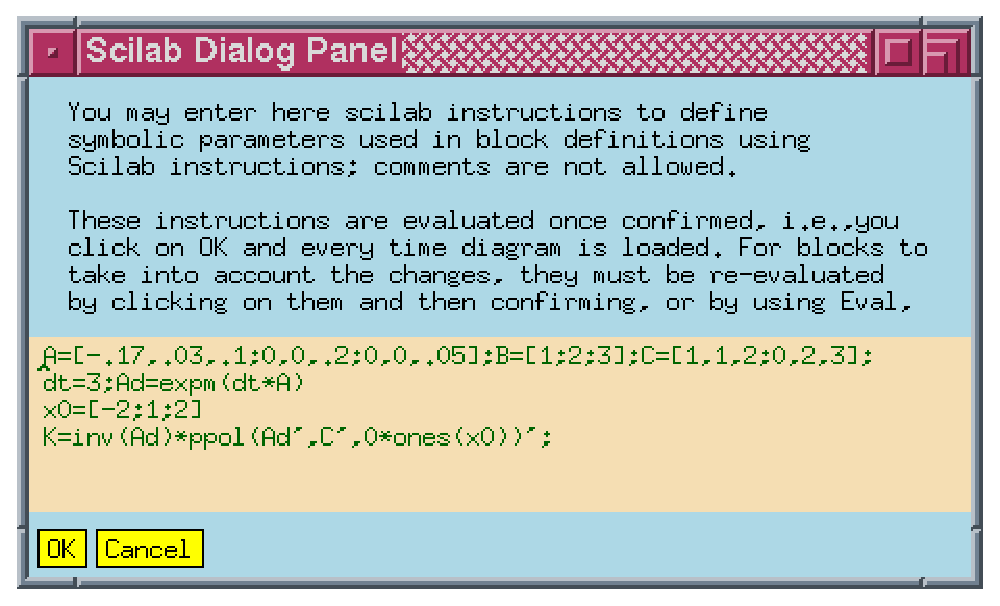
\epsfig{file=context_hyb.eps,width=11cm}}
 \caption{Context of the diagram.}
\label{context_hyb}
 \end{figure}

The corresponding Scicos diagram is given in
Figure~\ref{cont_disc_dia};  the observed system is the Super Block in
Figure~\ref{sysforhyb}) and the hybrid observer  is the Super Block in
Figure~\ref{hyb_obs_dia}).  

\input cont_disc_dia.tex
\dessin{Linear system with a hybrid observer}{cont_disc_dia}

\input sysforhyb.tex
\dessin{Model of the system. The two outputs are {\tt y} and {\tt
x}. The gain is {\tt C}.}{sysforhyb} 

\input hyb_obs_dia.tex
\dessin{Model of the hybrid observer. The two inputs are {\tt u} and {\tt
y}.}{hyb_obs_dia} 

The {\tt A}
and {\tt B} matrices are used both in the definition of the linear system 
and the {\tt Jump linear system} used in the two Super Blocks; the
difference is that in the case of 
the system, the initial condition {\tt x0} is used
(Figure~\ref{sysforhybdlg}) whereas in the case
of observer, the initial condition is set to zero. 
The {\tt C} and {\tt K} matrices are used 
in the {\tt Gain} blocks. In particular, the observer gain
is given in Figure~\ref{hybobsdlgdlg}. The {\tt dt} parameter is used
in the {\tt Clock}. The result of the simulation (which gives the
observation error of all the components of the state) is given in
Figure~\ref{cont_disc_osc}. 

%
  \begin{figure}[htbp]
  \centerline{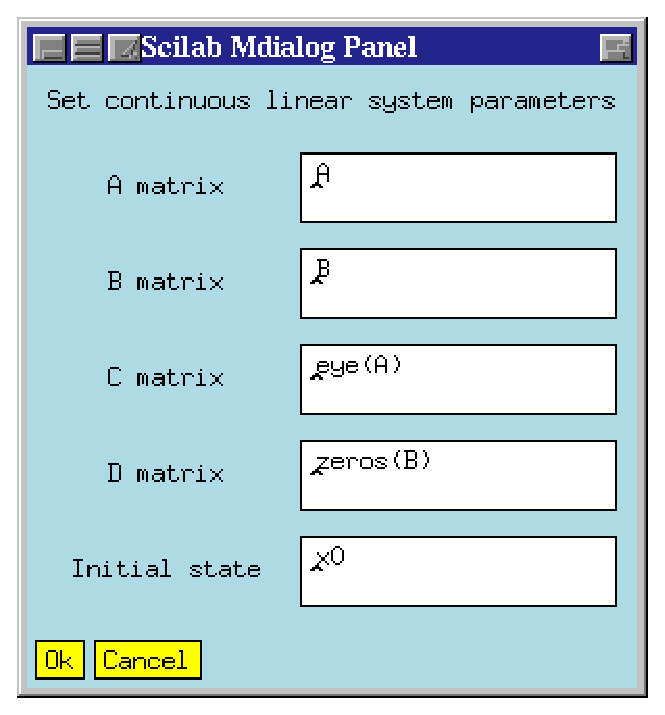
\epsfig{file=sysforhybdlg.eps,width=8cm}}
  \caption{Linear system dialogue box}
 \label{sysforhybdlg}
  \end{figure}

  \begin{figure}[htbp]
  \centerline{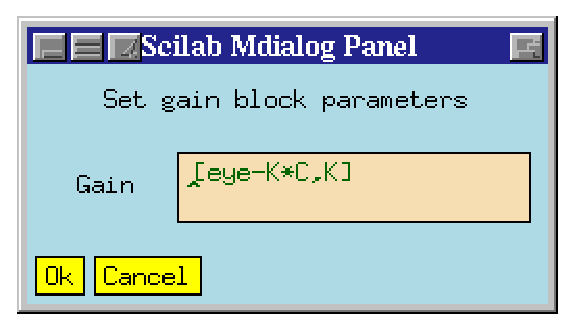
\epsfig{file=hybobsdlgdlg.eps,width=6cm}}
  \caption{{\tt Gain} block dialogue box}
 \label{hybobsdlgdlg}
  \end{figure}



\input cont_disc_osc.tex
\dessin{Simulation result.}{cont_disc_osc} 

Note that in this diagram, not only the system matrices, but also
their dimensions are arbitrary. You can for example change the {\tt C}
matrix so that the number of outputs of the system changes. 

This example is part of Scicos demos. You can experiment by changing
the context (don't forget to {\tt Eval} for your modifications to be
effective). 


\chapter{Future developments}
The development of Scicos is actively pursued. There are a number of
new features which should be operational in the near future. A few of
these developments are presented in this chapter.



\section{Different types of links and states}
In the current version of Scicos, all the link registers are coded
as ``double precision'' numbers. This means that for the moment, blocks
inputs and outputs cannot be of type integer, boolean, etc... In the
next version of Scicos, each link will have its own type 
(we are considering fortran types only, but that can be
changed). The link type is inherited from input and output types of
the blocks connected to it. This means that in defining
a block, in addition to specifying the size of each input and
output, the type of each input and output must also be specified.
The compiler of course verifies that ports of different types
are not connected together.

Similarly the discrete states will be allowed to be composed of
subsets of different types. The continuous states however
remain as they are.


\section{Real-time code generation}
To be able to generate real-time code for various processors
realizing Scicos diagrams, an interface to SynDEx is currently
being developed (for information on SynDEx, see
\cite{syndex1,syndex2}).

The objective is to have an environment where user can select
a portion of his Scicos diagram, usually coresponding to a
a discrete controller, click on a button and end up in SynDEx
environment loaded with the graph  corresponding
to this portion. From there,
user can generate optimized multi-processor real-time code
for almost any target processor.

\section{Blocks imposing implicit relations}
Currently, all the CBB's are explicit in a sense that they cannot
impose implicit constraints among signals on different ports;
there is clear distinction between inputs and outputs, even though
as far as memory management is concerned,   
inputs and outputs are handled in a completely analogous way in
Scicos. In a future version, it would be possible to define blocks
imposing implicit relations (algebraic constraints). This often leads
to having to solve differential-algebraic equations (DAE), for which we
shall use {\tt dassl} \cite{dassl1,dassl2} as solver. 


\appendix

\chapter{Using the graphical user interface}
\label{tta}
\section{Overview}
This section describes various functions of the graphical user
interface of Scicos. To invoke Scicos, user should type
\underline{{\tt scicos();}} 
in a regular Scilab session. This opens up a 
Scicos   window inside a Scilab graphics window. By default, this window is
entitled {\tt Untitled} and contains an empty model.

An existing model can be loaded at this point using the {\tt load}
button in {\tt File..} menu (this can also be done directly by
using the string containing the name of the file containing the
existing model, as argument of the {\tt scicos} command) or a new model can
be constructed in the {\tt Untitled} window. The model can be saved on
file in various formats. 

All the operations in Scicos  are done by
clicking on various buttons in the Scicos  windows. A detailed
description is given in Appendix~\ref{gui}. Description can also be obtained
on each button by clicking first on the {\tt Help}
button, then on the button in question. For help on blocks, user can click
first on the {\tt Help}, then on the block in question. 

The most common way of constructing Scicos   models is by using existing
blocks in Scicos' palettes. Click on the {\tt Palettes} button in the
{\tt edit..} menu to open
the palettes. In various palettes, user can find elementary blocks such as
addition, gain, multiplication, ..., linear system blocks (continuous,
discrete both in transfer function and state-space forms), nonlinear
blocks, input output devices (reading from and writing to file, scope,
...), event generating blocks (clock, event delay, ...) and more. Any
number of palettes can be open and active at any time.


\subsection{Blocks in palettes}
\label{pal}
Blocks in palettes can be copied into Scicos  window by clicking on the
{\tt Copy} button in the {\tt Edit..} menu, then on the block to be copied
and finally where the 
block is to be placed in Scicos window. See Tables~\ref{ttt1} 
through~\ref{ttte} for a list and a short description of available
blocks in different palettes.

\begin{table}[ht]
\begin{center}
\begin{tabular}{|c|c|l|} \hline
\interfacing function&\computational function&Short description\\
\hline
AFFICH\_f& affich.f  & display input value in diagram           \\
ANIMXY\_f& scopxy.f          &   animation; inputs are x-y coord.        \\
CLOCK\_f& {\em super block}          &  generate events periodically          \\
CONST\_f& cstblk.f          &   constant output         \\
CURV\_f&  intplt.f         &    signal defined by interpolation       \\
EVENTSCOPE\_f& evscpe.f          &  visualization of events          \\
GENSIN\_f& gensin.f          &   sinusoid generator         \\
GENSQR\_f&  gensqr.f         &  square wave generator          \\
MSCOPE\_f& mscope.f              &  multi-display scope            \\
RAND\_f&  rndblk.f         &  random generator          \\
RFILE\_f& readf.f          &  read form file          \\
SAWTOOTH\_f& sawtth.f          & sawtooth generator           \\
SCOPE\_f& scope.f          &   scope; one (vector) input         \\
SCOPXY\_f& scopxy.f          & plots second input as function of first           \\
TIME\_f&  timblk.f         &  output is time          \\
WFILE\_f& writef.f          & write to file           \\ \hline
\end{tabular}
\end{center}
\caption{Blocks in Inputs\_Outputs palette}
\label{ttt1}
\end{table}

\begin{table}[ht]
\begin{center}
\begin{tabular}{|c|c|l|} \hline
\interfacing function&\computational function&Short description\\
\hline
CLR\_f&  csslti.f         & cont. lin. sys. (transfer function)           \\
CLSS\_f& csslti.f          & cont. lin. sys. (state space)            \\
DELAYV\_f&delayv.f           & variable delay           \\
DELAY\_f& {\em super block}          & fixed delay           \\
DLR\_f&   dsslti.f        &  discr. lin. sys. (transfer function)          \\
DLSS\_f&  dsslti.f         &  discr. lin. sys. (state space)            \\
DOLLAR\_f& dollar.f              & single scalar register               \\
GAIN\_f&  gain.f         &   matrix gain         \\
INTEGRAL\_f&  integr.f         &   scalar integrator         \\
REGISTER\_f& delay.f          &   shift register         \\
SAMPLEHOLD\_f& samphold.f          &   sample and hold block         \\
SOM\_f& sum2 {\em and} sum3          &  addition          \\
TCLSS\_f&tcslti.f           & cont. lin. sys. with jump           \\ \hline
\end{tabular}
\end{center}
\caption{Blocks in Linear palette}
\end{table}

\begin{table}[ht]
\begin{center}
\begin{tabular}{|c|c|l|}\hline
\interfacing function&\computational function&Short description\\
\hline
ABSBLK\_f&absblk.f&abs value of vector \\
COSBLK\_f& cosblk.f          &   cosine operation         \\
DLRADAPT\_f& dlradp.f          &            \\
EXPBLK\_f& expblk.f          &   exponentiation         \\
INVBLK\_f&  invblk.f         &     inversion       \\
LOGBLK\_f& logblk.f          &     logarithm       \\
LOOKUP\_f&  lookup.f         &   lookup table         \\
MAX\_f&  maxblk.f         &      maximum of inputs      \\
MIN\_f&  minblk.f         &     minimum of inputs       \\
POWBLK\_f& powblk.f           &   computes to the power of         \\
PROD\_f&  prod.f         &      multiplication      \\
QUANT\_f& qzrnd.f          &            \\
SAT\_f&   lusat.f        &   saturation         \\
SINBLK\_f& sinblk.f          &      sine operation      \\
TANBLK\_f& tanblk.f          &    tangent operation        \\ \hline   
\end{tabular}
\end{center}
\caption{Blocks in Non Linear palette}
\end{table}

\begin{table}[ht]
\begin{center}
\begin{tabular}{|c|c|l|}\hline
\interfacing function&\computational function&Short description\\
\hline
ANDLOG\_f& andlog.f          &            \\
EVTGEN\_f& {\em none}          &   generates event at specified time         \\
EVTDLY\_f& evtdly.f          &     delay on event       \\
HALT\_f&  hltblk.f         &   stop simulation if event received         \\
MCLOCK\_f& {\em super block}          &   multi frequency clock         \\
MFCLCK\_f&  mfclck         &            \\
TRASH\_f& trash.f          &   does nothing         \\ \hline   
\end{tabular}
\end{center}
\caption{Blocks in Events palette}
\end{table}

\begin{table}[ht]
\begin{center}
\begin{tabular}{|c|c|c|c|}\hline
\interfacing function&\computational function&Short description\\
\hline
GENERAL\_f& zcross.f          & detects conditional zero crossing           \\
NEGTOPOS\_f& zcross.f          &   zero crossing with positive slope         \\
POSTONEG\_f&   zcross.f           &  zero crossing with negative slope         \\
ZCROSS\_f& zcross.f          &    detects zero crossing     \\ \hline   
\end{tabular}
\end{center}
\caption{Blocks in Treshold palette}
\end{table}

\begin{table}[ht]
\begin{center}
\begin{tabular}{|c|c|c|c|}\hline
\interfacing function&\computational function&Short description\\
\hline
scifunc\_block& {\em generated}          &  used to define blocks in Scilab          \\
generic\_block& {\em user supplied}      &  generic \interfacing function          \\
SUPER\_f& {\em super block}          &            \\   
TEXT\_f& text.f          &    used to include text in diagram        \\ \hline 
\end{tabular}
\end{center}
\caption{Blocks in Others palette}
\end{table}


\begin{table}[ht]
\begin{center}
\begin{tabular}{|c|c|c|} \hline
\interfacing function&\computational function&Short description\\ \hline
DEMUX\_f& demux.f          &  one vector input demultiplexed          \\
ESELECT\_f&   eselect.f                 &  input event directed to one output      \\
IFTHEL\_f&  ifthel.f         &            \\
MUX\_f&  mux.f         &inputs multiplexed to one output            \\
SELECT\_f&   selector.c        &   one of regular inputs gets out         \\ \hline 
\end{tabular}
\end{center}
\caption{Blocks in Branching palettes}
\label{ttte}
\end{table}

By clicking on a block in
Scicos window, a dialog opens up and the user can set block parameters. 
Help on a block can be obtained by clicking on the {\tt Help} button,
then on the block (in the palette or in the Scicos   window).

Event input ports are always placed on top, and event output ports on the
bottom. regular input and output ports however can be placed on either
side. User can use the {\tt Flip} button to change the places of input and
output ports. The regular input and output ports are numbered from top to
bottom, and the event input and output ports, from left to right
(whether or not the block is flipped).

\subsection{Connecting blocks}
Connecting blocks can be accomplished by clicking on the {\tt Link}
button in the {\tt Edit..} menu, then on the output port and then the
input port. This makes a 
straight line connection. For more complex connections, before
clicking on the input port, user can click on intermediary points on
Scicos   window, to guide the path. Whenever possible, Scicos   draws
perfectly horizontal or vertical paths. Obviously only output ports
and input ports of the same type can be connected. The color of the
path can be changed by clicking on the path.

For some blocks, the number of inputs and outputs ports may depend on block
parameters. In this case,
user should adjust block parameters before connecting its ports (it is
not possible to remove connected ports). 

A path can originate from a path, i.e., a path can be split, by clicking
on the {\tt Link} button and then on an existing path, where split is
to be placed, and finally on an input port (or intermediary points
before that). 

\subsection{How to correct mistakes}
If a block is not correctly placed it can be moved. This can be done
by clicking on the {\tt Move} button (in the {\tt Edit..} menu) first,
then by clicking on the block to be moved, dragging the block
to the desired location where a last click fixes the position (pointer
position corresponds to the lower left corner of the block box).

If a block or a path is not needed, it can be removed using the {\tt
Delete} Button. This can be done by clicking first on {\tt Delete}
and then clicking left on the object to be removed (or right to delete
a region). If a block is
removed, all paths connected to this block are also removed. 

If an incorrect editing operation is performed, it can be taken back. See
help on the {\tt Undo} button.

\subsection{Save model and simulate}
Once the Scicos   model is constructed, it can be saved, compiled and 
simulated. Normally a finished model should not contain any
unconnected input ports (if some regular input ports are left unconnected, the
corresponding blocks are deactivated).
To simulate the model, user should click on the {\tt Run} button in
the {\tt Simulation..} menu. Simulation parameters can be set before using
the {\tt setup} button. 

System parameters can be modified in the course of the simulation.
Clicking on {\tt Stop} button on top of the main Scicos  window halts the
simulation and activates the Scicos 
panel. The system can then be modified and the simulation 
continued or restarted by clicking on the {\tt Run} button. The
compilation is done automatically if needed. If after a modification
the simulation does not work properly, a manual compilation ({\tt
Compile} button) may be necessary. Such situations should be reported.


\subsection{Editing palettes}
Scicos provides a number of predefined palettes (see Section~\ref{pal}). The
Palette editor can be used to create and modify new palettes.
To use it, user should click on the 
{\tt Pal editor..} button of the main Scicos menu. A new 
window appears with a menu similar to Scicos' main menu. This is the
Palette editor.

\paragraph{Creating and modifying a palette}
To modify an existing palette, user should load it in the
Palette editor window by clicking first on {\tt File..} and then {\tt
Load} (Scicos predefined palettes
may be found in {\tt <SCIDIR>/macros/scicos/*.cosf } files).
It is then possible to copy blocks from palettes or from main Scicos 
window using  {\tt Copy} button in the {\tt Edit..} menu, or
add newly defined blocks. For that, user should click on the
{\tt AddNew} button in the {\tt Edit..} menu (in the Palettes editor mode).
A dialogue box inquires then the name of the \interfacing function
associated with 
the new block.\footnote{Not the name of the file that contains it.}

If the \interfacing function is not yet defined in Scilab,
a file selection dialogue opens up and user is requested to select
the file that contains it; in this case the corresponding 
{\tt getf} instruction needed to load the function for further use 
is added automatically to the {\tt .scilab} startup file in user's
home directory. 

To have modifications taken into account user should save the modified
palette (using {\tt Save} if it has the desired name, or
{\tt Save As} or {\tt FSave} buttons in the {\tt File..} menu) before
leaving the Palette edition mode (using {\tt Exit} button).

Creating a new palette can be done exactly the same way (except that
there is no palette to load initially). At the end, Scicos attempts to
customize user's {\tt .scilab} startup file by adding the path and
the name of the new palette and if necessary the instructions necessary
to get block \interfacing functions (user is asked to confirm or
refuse these modifications). 


\paragraph{Converting a Super Block into a block}
If user wants to freeze a Super block in a single block before adding
it to a palette, he should first click on it to open the Super block's
diagram. Then it must click on the {\tt Newblk} button in the {\tt
File..} menu. A dialogue box will appear asking user to set the path
of the directory where he wants to place the file containing the
new block's \interfacing function. The name of the created file is {\tt
<path><window name>.sci}. To change the window name before freezing
the Super block, it is necessary to save the super block in a file
using {\tt Save As} button in the {\tt File..} menu.

Once frozen, Super block's structure cannot be changed. 
Clicking on itk opens one after the other, all {\tt set} dialogues of
every block present in the Super block.

It is
possible to recover the Super block by modifying (using a text editor)
the generated \interfacing function  by replacing the {\tt 'csuper'}
character string by {\tt 'super'} in {\tt model(1)} definition.

\chapter{Reference guide}
\label{gui}
\input ../LaTex-doc/Chap2-5.tex

\begin{thebibliography}{99}
\bibitem{simulink} {\em SIMULINK User's guide}, The MathWorks, Inc., 1993.
\bibitem{systembuild} {\em SystemBuild User's Guide}, Integrated Systems
Inc., 1994.
\bibitem{Hybrid} Grossman, R. L., Nerode A., Ravn, A. P. and Rischel H. (Eds.),
{\em Hybrid Systems}, Lecture Notes in Computer Science 736, Springer
Verlag, Berlin Heidelberg, 1993.
\bibitem{mats} Andersson, M., {\em Object-oriented modeling and
simulation of hybrid systems}, Ph. D. Thesis, Lund Institute of
Technology, 1994.
\bibitem{ls1} Hindmarsh, A. C.,  ``Lsode and Lsodi, two new initial value
ordinary differential equation solvers,'' {\em
ACM-Signum Newsletter}, vol. 15, no. 4, 1980.
\bibitem{ls2} Petzold, L. R., ``Automatic selection of methods for solving
stiff and nonstiff systems of ordinary differential equations,''
{\em SIAM J. Sci. Stat. comput.}, 4, 1983.
\bibitem{dassl1} Petzold, L. R., ``A description of DASSL: a
differential/algebraic system solver,'' in {\em Scientific Computing},
eds. R. S. Stepleman et al., North-Holland, 1983.
\bibitem{dassl2} Brenan, K. E., Campbell, S. L., and Petzold, L. R.,
{\em Numerical Solution of Initial-Value Problems in
Differential-Algebraic Equations}, North-Holland, 1989.
\bibitem{syndex1}
Sorel, Y., ``Real-time embedded image processing applications using
the A3 methodology,'' 
{\em Proc. IEEE Internat. Conf. Image Processing}, Lausanne, Switzerland, Sept. 1996.

\bibitem{syndex2}
Sorel, Y., ``Massively Parallel Computing Systems with Real-Time
Constraints: 
the Algorithm Architecture Adequation Methodology,''
{\em Proc. Conf. MPCS94}, Ischia, Italy, May 1994.

\end{thebibliography}



\end{document} 
